
\section{HÀM SỐ MŨ. HÀM SỐ LOGARIT}

\subsection{Tóm tắt lý thuyết}
\begin{tomtat}
\subsubsection{Định nghĩa}
\begin{dn}
	Cho số dương $a$ khác $1$. Hàm số cho tương ứng mỗi số thực $x$ với số thực $a^x$ được gọi là \textbf{hàm số mũ} cơ số $a$, kí hiệu $y=a^x$.
\end{dn}
\textbf{Nhận xét:} Hàm số $y=a^x$ có tập xác định là $\mathbb{R}$.	
\begin{dn}
	Đồ thị hàm số $y=a^x$ $(a>0, a \neq 1)$ là một đường cong liền nét, cắt trục tung tại điểm có tung độ bằng $1$, nằm ở phía trên trục hoành và đi lên nếu $a>1$, đi xuống nếu $0<a<1$.
\end{dn}

\begin{center}
	\begin{tikzpicture}[>=stealth,line join=round,line cap=round,font=\footnotesize,scale=0.5]
		\def\a{2}
		\draw[->] (-5,0) -- (5,0) node[below] {$x$};
		\draw[->] (0,-2) -- (0,5) node[left] {$y$};
		\draw (0,0)node[below left]{$O$};
		\clip (-5,-1)rectangle(5,5);
		\draw[thick,samples=200,smooth,domain=-4.5:4.5] plot(\x, {\a^\x});
		\draw[dashed] (0,2)--(1,2)--(1,0);
		\draw (0,1) node [above left=-0.1] {$1$};
		\draw (0,2) node [left=-0.05] {$a$};
		\draw (1,0) node [below] {$1$};
		\draw (2.2,4.5) node [right] {$y=a^x$};
		\draw (2,3.8) node [right] {$(a>1)$};
	\end{tikzpicture}
	\qquad
	\begin{tikzpicture}[>=stealth,line join=round,line cap=round,font=\footnotesize,scale=0.5]
		\def\a{0.5}
		\draw[->] (-5,0) -- (5,0) node[below] {$x$};
		\draw[->] (0,-2) -- (0,5) node[left] {$y$};
		\draw (0,0)node[below left]{$O$};
		\clip (-5,-1)rectangle(5,5);
		\draw[thick,samples=200,smooth,domain=-4.5:4.5] plot(\x, {\a^\x});
		\draw[dashed] (0,0.5)--(1,0.5)--(1,0);
		\draw (0,1) node [above right=-0.1] {$1$};
		\draw (0,0.5) node [left=-0.05] {$a$};
		\draw (1,0) node [below] {$1$};
		\draw (-4.4,4.5) node [right] {$y=a^x$};
		\draw (-4.3,3.8) node [right] {$(a<1)$};
	\end{tikzpicture}
\end{center}

\textbf{Nhận xét:} Cho hàm số mũ $y=a^x$ $(a>0, a\ne 1)$.\\
\begin{center}
	\begin{tabular}{|c|c|}\hline
		$y=a^x$ $(a>1)$&$y=a^x$ $(0<a<1)$\\ \hline
		$\mathscr{D}=\mathbb{R}$; $T=(0;+\infty)$. & $\mathscr{D}=\mathbb{R}$, $T=(0;+\infty)$.\\\hline
		Tính liên tục: Hàm số liên tục trên $\mathbb{R}$.& Tính liên tục: Hàm số liên tục trên $\mathbb{R}$.\\\hline
		Giới hạn đặc biệt&Giới hạn đặc biệt\\
		$\lim\limits_{x \rightarrow-\infty} a^x=0, \lim\limits_{x \rightarrow+\infty} a^x=+\infty$.& $\lim\limits_{x \rightarrow-\infty} a^x=+\infty, \lim\limits_{x \rightarrow+\infty} a^x=0$.\\\hline
		Sự biến thiên: Hàm số đồng biến trên $\mathbb{R}$.& Sự biến thiên: Hàm số nghịch biến trên $\mathbb{R}$.\\\hline
		Bảng biến thiên & Bảng biến thiên\\
		\qquad
\begin{tikzpicture}[>=stealth,line join=round,line cap=round,font=\footnotesize,scale=1]
			\tkzTabInit[nocadre=false,lgt=1.7,espcl=1.5,deltacl=0.5]{$x$/0.7,$y=a^x$/2}
			{$-\infty$ , $0$ , $+\infty$}
			\tkzTabVar{-/$0$ , R , +/$+\infty$}
			\tkzTabIma{1}{3}{2}{$1$}% Từ cột 1 đến cột 3 đặt f(2) tại cột 2.
		\end{tikzpicture}
		&\qquad
\begin{tikzpicture}[>=stealth,line join=round,line cap=round,font=\footnotesize,scale=1]
			\tkzTabInit[nocadre=false,lgt=1.7,espcl=1.5,deltacl=0.5]{$x$/0.7,$y=a^x$/2}
			{$-\infty$ , $0$ , $+\infty$}
			\tkzTabVar{+/$+\infty$ , R , -/$0$}
			\tkzTabIma{1}{3}{2}{$1$}% Từ cột 1 đến cột 3 đặt f(2) tại cột 2.
		\end{tikzpicture}
		\\\hline
	\end{tabular}
\end{center}
% \begin{note}
% 	\immini{Từ tính liên tục và sự biến thiên của hàm số mũ, ta có thể chứng minh được mệnh đề sau:
% 		Với mỗi $N>0$, đường thẳng $y=N$ cắt đồ thị hàm số mũ $y=a^x$ $(a>0, a \neq 1)$ tại một và chỉ một điểm (Hình bên). Nói cách khác, ta có: Với mỗi $N>0$, tồn tại duy nhất số thực $\alpha$ sao cho $a^\alpha=N$.}{\begin{tikzpicture}[>=stealth,line join=round,line cap=round,font=\footnotesize,scale=0.5]
% 			\def\a{2}
% 			\draw[->] (-5,0) -- (5,0) node[below] {$x$};
% 			\draw[->] (0,-2) -- (0,5) node[left] {$y$};
% 			\draw (0,0)node[below left]{$O$};
% 			\clip (-5,-1)rectangle(5,5);
% 			\draw[thick,samples=200,smooth,domain=-4.5:4.5] plot(\x, {\a^\x});
% 			\draw[dashed] (0,2)--(1,2)--(1,0);
% 			\draw (0,1) node [above left=-0.1] {$1$};
% 			\draw (0,2) node [above left=-0.05] {$N$};
% 			\draw (1,0) node [below] {$\alpha$};
% 			\draw (2.2,4.5) node [right] {$y=a^x$};
% 			\draw (-3,2)--(4,2)node[above] {$y=N$};
% 	\end{tikzpicture}}
% \end{note}	
	
\begin{dn}
	Cho số dương $a$ khác $1$. Hàm số cho tương ứng mỗi số thực dương $x$ với số thực $\log_ax$ được gọi là \textbf{hàm số lô-ga-rít} cơ số $a$, kí hiệu $y=\log_ax$.
\end{dn}

\textbf{Nhận xét:} Cho hàm số $y=\log_a x$ $(a>0, a\ne 1)$.\\
\begin{center}
	\begin{tabular}{|c|c|}\hline
		$y=a^x$ $(a>1)$&$y=a^x$ $(0<a<1)$\\ \hline
		$\mathscr{D}=(0;+\infty)$; $T=\mathbb{R}$ & $\mathscr{D}=(0;+\infty)$; $T=\mathbb{R}$.\\\hline
		Tính liên tục: Hàm số liên tục trên $(0;+\infty)$.& Tính liên tục: Hàm số liên tục trên $(0;+\infty)$.\\\hline
		Giới hạn đặc biệt& Giới hạn đặc biệt\\
		$\lim\limits_{x\to+\infty}\log_ax=+\infty$, $\lim\limits_{x\to0^+}\log_ax=-\infty$ & $\lim\limits_{x\to+\infty}\log_ax=-\infty$, $\lim\limits_{x\to0^+}\log_ax=+\infty$.\\\hline
		Hàm số đồng biến trên $(0;+\infty)$.&Hàm số nghịch biến trên $(0;+\infty)$.\\\hline
		Bảng biến thiên &  Bảng biến thiên\\
			
\begin{tikzpicture}[>=stealth,line join=round,line cap=round,font=\footnotesize,scale=1]
				\tkzTabInit[nocadre=false,lgt=2,espcl=1.5,deltacl=0.5]{$x$/0.7,$y=\log_ax$/2}
				{$0$ , $1$ , $+\infty$}
				\tkzTabVar{-/$-\infty$ , R , +/$+\infty$}
				\tkzTabIma{1}{3}{2}{$0$}% Từ cột 1 đến cột 3 đặt f(2) tại cột 2.
			\end{tikzpicture}
		& 
\begin{tikzpicture}[>=stealth,line join=round,line cap=round,font=\footnotesize,scale=1]
					\tkzTabInit[nocadre=false,lgt=2,espcl=1.5,deltacl=0.5]{$x$/0.7,$y=\log_ax$/2}
					{$0$ , $1$ , $+\infty$}
					\tkzTabVar{+/$+\infty$ , R , -/$-\infty$}
					\tkzTabIma{1}{3}{2}{$0$}% Từ cột 1 đến cột 3 đặt f(2) tại cột 2.
				\end{tikzpicture}
		\\\hline
	\end{tabular}
\end{center}

% \begin{note}
% 	Hàm số $y=\log_ax$, $a>0$, $a\ne1$ có
% 	\begin{itemize}
% 		\item Tập xác định là $\mathscr{D}=(0;+\infty)$.\\
% 		Tập giá trị là $T=\mathbb{R}$.\\
% 		Hàm số liên tục trên $(0;+\infty)$.
% 		\item Sự biến thiên:
% 		\begin{itemize}
% 			\item Nếu $a>1$ thì hàm số đồng biến trên $(0;+\infty)$ và $\lim\limits_{x\to+\infty}y=\lim\limits_{x\to+\infty}\log_ax=+\infty$, $\lim\limits_{x\to0^+}y=\lim\limits_{x\to0^+}\log_ax=-\infty$.\\
% 			Bảng biến thiên\begin{center}
% 				\begin{tikzpicture}[>=stealth,line join=round,line cap=round,font=\footnotesize,scale=1]
% 					\tkzTabInit[nocadre=false,lgt=2.3,espcl=2,deltacl=0.5]{$x$/0.7,$y=\log_ax$/2}
% 					{$0$ , $1$ , $+\infty$}
% 					\tkzTabVar{-/$-\infty$ , R , +/$+\infty$}
% 					\tkzTabIma{1}{3}{2}{$0$}% Từ cột 1 đến cột 3 đặt f(2) tại cột 2.
% 				\end{tikzpicture}
% 			\end{center}
% 			\item Nếu $0<a<1$ thì hàm số nghịch biến trên $(0;+\infty)$ và $\lim\limits_{x\to+\infty}y=\lim\limits_{x\to+\infty}\log_ax=-\infty$, $\lim\limits_{x\to0^+}y=\lim\limits_{x\to0^+}\log_ax=+\infty$.\\
% 			Bảng biến thiên
% 			\begin{center}
% 				\begin{tikzpicture}[>=stealth,line join=round,line cap=round,font=\footnotesize,scale=1]
% 					\tkzTabInit[nocadre=false,lgt=2.3,espcl=2,deltacl=0.5]{$x$/0.7,$y=\log_ax$/2}
% 					{$0$ , $1$ , $+\infty$}
% 					\tkzTabVar{+/$+\infty$ , R , -/$-\infty$}
% 					\tkzTabIma{1}{3}{2}{$0$}% Từ cột 1 đến cột 3 đặt f(2) tại cột 2.
% 				\end{tikzpicture}
% 			\end{center}
% 		\end{itemize}
% 		\item Đồ thị của hàm số
% 		\begin{itemize}
% 			\item Cắt trục hoành tại điểm $(1;0)$, đi qua điểm $(a;1)$.
% 			\item Nằm bên phải trục tung.
% 		\end{itemize}	
		\begin{center}
			\begin{tikzpicture}[>=stealth,line join=round,line cap=round,font=\footnotesize,scale=0.7]
				\draw[->](-1,0) -- (5,0) node[below]{ $x$};
				\draw[->](0,-3) -- (0,4) node[below,right]{ $y$};
				\draw(-0.2,0) node[below left]{\footnotesize $O$};
				\clip(-1,-3) rectangle (5,4);
				\draw[smooth,domain=0.05:4.5]plot(\x,{ln(\x)/ln(2)});
				\draw(1,0) node[below]{ $1$};
				\draw[dashed] (0,1) node[left]{$1$}--(2,1)--(2,0)node[below]{$a$};
				\draw (0.3,-1.6)node[right]{$y=\log_ax$ $(a>1)$};
			\end{tikzpicture}
			\qquad
			\begin{tikzpicture}[>=stealth,line join=round,line cap=round,font=\footnotesize,scale=0.7]
				\draw[->](-1,0) -- (5,0) node[below]{\footnotesize $x$};
				\draw[->](0,-3) -- (0,4) node[below,right]{\footnotesize $y$};
				\draw(-0.2,0) node[below left]{\footnotesize $O$};
				\clip(-1,-3) rectangle (6,4);
				\draw[smooth,domain=0.07:4.5]plot(\x,{-ln(\x)/ln(2)});
				\draw(1,0) node[below]{ $1$};
				\draw[dashed] (0,1) node[left]{$1$}--(1/2,1)--(1/2,0)node[below]{$a$};
				\draw (0.1,3)node[right]{$y=\log_ax$ $(0<a<1)$};
			\end{tikzpicture}
		\end{center}
% 	\end{itemize}
% \end{note}	
	
\end{tomtat}
\setcounter{subsubsection}{0}
\setcounter{ex}{0}
\setcounter{bt}{0}
\subsection{Các dạng toán thường gặp}


\begin{dang}{Tập xác định của hàm số}
 Hàm số $y=\log_af(x)$ ($0<a\ne 1$) xác định khi $f(x)>0$.
\end{dang}

\subsubsection{Ví dụ mẫu}
\begin{vd}%%[CD]%[Đỗ Minh Phúc]%[1C6B3-1]
	Tìm tập xác định của hàm số $y=12^x$.
	\loigiai{
	Tập xác định của hàm số $y=12^x$ là $\mathscr{D}=\mathbb{R}$.
	}
\end{vd}

\begin{vd} %[Tex hóa SGK CD-CT,T7/22, TVN-019]%[1T6B3-1]
	Tìm tập xác định của các hàm số
	\begin{enumEX}{2}
		\item $y=\log_2(3-2x)$.
		\item $y=\log_3\left(x^2+4x\right)$.
	\end{enumEX}
	\loigiai{\begin{enumerate}
			\item Hàm số $y=\log_2(3-2x)$ xác định khi $3-2x>0\Leftrightarrow x<\dfrac{3}{2}$.\\
			Vậy tập xác định của hàm số $y=\log_2(3-2x)$ là $\mathscr{D}=\left(-\infty;\dfrac{3}{2}\right)$.
			\item Hàm số $y=\log_3\left(x^2+4x\right)$ xác định khi $x^2+4x>0\Leftrightarrow x<-4\vee x>0$.\\
			Vậy tập xác định của hàm số $y=\log_3\left(x^2+4x\right)$ là $\mathscr{D}=(-\infty;-4)\cup(0;+\infty)$.
	\end{enumerate}}
\end{vd}
\begin{vd} %[Tex hóa SGK CD-CT,T7/22, TVN-001]%[1K6YI-1]
	Tìm tập xác định của các hàm số sau
	\begin{multicols}{2}
		\begin{enumerate}
			\item $y = \log |x+3|$ ;
			\item $y = \ln (4-x^{2})$.
		\end{enumerate}
	\end{multicols}
	\loigiai{
		\begin{enumerate}
			\item Hàm số xác định khi và chỉ khi $x+3 \neq 0$ hay $x \neq  -3$. \\
			Suy ra tập xác định $\mathscr D = \mathbb{R} \setminus \{-3\}$.
			\item Hàm số xác định khi và chỉ khi $4-x^2>0$ hay $-2<x<2$. \\
			Suy ra tập xác định $\mathscr D = \left( -2; 2 \right)$.
		\end{enumerate}
		
	}
\end{vd}

\begin{vd}%%[CD]%[Đỗ Minh Phúc]%[1C6B3-1]
	Tìm tập xác định của các hàm số
	\begin{multicols}{2}
		\begin{enumerate}
			\item $y=\log_5(2 x-3)$;
			\item $y=\log_{\tfrac{1}{5}}\left(-x^2+4\right)$.
		\end{enumerate}
	\end{multicols}
	\loigiai{
		\begin{enumerate}
			\item Điều kiện $2x-3>0\Leftrightarrow x>\dfrac{3}{2}$.\\
			Vậy tập xác định của hàm số $y=\log_5(2x-3)$ là $\mathscr{D}=\left(\dfrac{3}{2};+\infty \right) $.
			\item Điều kiện $-x^2+4>0\Leftrightarrow -2<x<2$.\\
			Vậy tập xác định của hàm số $y=\log_{\tfrac{1}{5}}\left(-x^2+4\right)$ là $\mathscr{D}=(-2;2)$.
		\end{enumerate}
	}
\end{vd}

\subsubsection{Bài tập rèn luyện}
\begin{bt}Tìm tập xác định của các hàm số sau
	\begin{multicols}{3} 	
	\begin{enumerate}
		\item $y=\log_6(x-4)$
		\item $y=\log_5(2x-1)$
		\item $y=\log _2(3-2 x)$
		\item $ y=\log_{2021}(3-x) $ 
		\item $y=\log_2(x-x^2)$
		\item $y=\log_3(x-4)$
		\item $y=\log_{7}(x+2)^2$
		\item $y=\log \left(2+x-x^2\right)$
		\item $y= \log_{2022} \left( 3x-x^2\right)$
		\item $y=\log_2\left(\dfrac{x-6}{1+x} \right)$
	\end{enumerate}
	\end{multicols}
	\loigiai{
		\begin{enumerate}
			\item Hàm số $y=\log_6(x-4)$ xác định khi và chỉ khi $x-4>0\Leftrightarrow x>4$.\\
			Vậy tập xác định $\mathscr{D}=(4;+\infty)$.
			\item Điều kiện xác định $2x-1>0\Leftrightarrow x>\dfrac{1}{2}$.\\
			Vậy tập xác định của hàm số đã cho là $\mathscr{D}=\left(\dfrac{1}{2};+\infty\right)$.
			\item Biểu thức $\log _2(3-2 x)$ có nghĩa $\Leftrightarrow x<\dfrac{3}{2}$.\\
			Vậy tập xác định của hàm số $y=\log _2(3-2 x)$ là	$\mathscr{D}=(-\infty;\dfrac{3}{2})$.	
			\item Điều kiện $ 3-x>0\Leftrightarrow x<3 $.\\
			Tập xác định của hàm số $ \mathscr{D}=(-\infty;3) $.
			\item Điều kiện $x-x^2>0\Leftrightarrow x\in (0;1)$.\\
			Tập xác định là $\mathscr{D}=(0;1)$.
			\item 	Điều kiện $x-4>0\Leftrightarrow x>4$.\\
			Vậy tập xác định là $\mathscr{D}=\left(4;+\infty\right)$.
			\item 	Hàm số xác định khi $(x+2)^2>0$. Điều này đúng với mọi $x \neq -2$.\\
			Tập xác định $\mathscr{D}=\mathbb{R} \setminus \{-2\}$.
			\item Hàm số $y=\log \left(2+x-x^2\right)$ xác định khi $ -x^2+x+2>0\Leftrightarrow -1<x<2 $.
			\\
			Tập xác định là $(-1 ; 2)$.
			\item 	Điều kiện xác định $3x-x^2>0 \Leftrightarrow 0<x<3$.\\
			Vậy tập xác định của hàm số đã cho là $D= (0; 3)$.
			\item Hàm số xác định khi và chỉ khi
			\[\dfrac{x-6}{x+1}>0 \Leftrightarrow \hoac{&x<-1\\&x>6.}\]
			Vậy tập xác định của hàm số là $\mathscr{D}=(-\infty;-1)\cup (6;+\infty)$.
		\end{enumerate}
		
		
	}
\end{bt}
\begin{bt} Tìm tất cả giá trị của tham số $m$ để hàm số sau xác định trên $\mathbb{R}$
	\begin{multicols}{2} 
	\begin{enumerate}
		\item $y=\log_2\left(x^2-2x+m\right)$
		\item $y=\log\left(x^2-2x-m+1\right)$
		\item  $y=\log_7\left(x^2-2x-m^2+5\right)$
		\item  $y=\ln \left( 3x^2+12mx+6\right) $
		\item $y=\log \left(x^2-8 x+10 m-m^2\right)$ 
	\end{enumerate}
\end{multicols}
	\loigiai{
		\begin{enumerate}
			\item Để hàm số $y=\log_2\left(x^2-2x+m\right)$ có tập xác định là $\mathbb{R}$ thì:
			$$x^2-2x+m>0,\forall x\in \mathbb{R}\Leftrightarrow \Delta '=1-m<0\Leftrightarrow m>1.$$
			\item 	Hàm số có tập xác định là $\mathbb{R}$  khi và chỉ khi $x^2-2x-m+1>0$, $\forall x \in \mathbb{R}$.\\
			Điều đó tương đương $\Delta'<0 \Leftrightarrow (-1)^2-(-m+1)<0 \Leftrightarrow m<0$.
			\item Điều kiện: $x^2-2x-m^2+5>0$.\\
			Hàm số đã cho có tập xác định là $\mathbb{R}$ khi và chỉ khi	$x^2-2x-m^2+5>0$, $\forall x\in\mathbb{R}$.
			$$\Leftrightarrow \heva{& a>0 \\ & \Delta'<0}\Leftrightarrow \heva{& 1>0 \\ & m^2-4<0}\Leftrightarrow -2<m<2.$$
			\item 	Hàm số xác định trên $\mathbb R$ khi và chỉ khi 
			\begin{eqnarray*}
				&& 3x^2+12mx+6>0, \;\forall x\in\mathbb R\\
				&\Leftrightarrow& \Delta'=(6m)^2-3\cdot 6<0\\
				&\Leftrightarrow& 36m^2-18<0\\
				&\Leftrightarrow& -\sqrt{\dfrac{1}{2}}<m<\sqrt{\dfrac{1}{2}}.
			\end{eqnarray*}
			\item Điều kiện để hàm số xác định trên 
			$\mathbb{R}$ là $$ x^2-8 x+10 m-m^2>0\, \forall x\in\mathbb{R}\Leftrightarrow \Delta'=m^2-10m+16<0 \Leftrightarrow 2<m<8.$$
		\end{enumerate}
		
		
	}
\end{bt}


\subsubsection{Bài tập trắc nghiệm}
\Opensolutionfile{ans}[ans/ans-Bai3-Dang1]
\begin{ex}
	Tập xác định của hàm số $y=\left(2-\sqrt{3}\right)^x$ là
	\choice
	{$(0;+\infty)$}
	{\True $(-\infty;+\infty)$}
	{$[0;+\infty)$}
	{$(-\infty;0)$}
	\loigiai
	{
		Tập xác định của hàm số $y=\left(2-\sqrt{3}\right)^x$ là $(-\infty;+\infty)$.
	}
\end{ex}


\begin{ex}
	Tập xác định của hàm số $y=7^x$ là
	\choice
	{$(0;1)$}
	{\True $(-\infty;+\infty)$}
	{$(0;+\infty)$}
	{$(1;+\infty)$}
	\loigiai
	{
		Hàm số $y=7^x$ xác định với mọi $x\in \mathbb{R}$. Do đó tập xác định $\mathscr{D}=\mathbb{R}$.
	}
\end{ex}



\begin{ex}
	Tìm tập xác định $\mathscr{D}$ của hàm số $y=\log_2\left(x^2-2x-3 \right) $.
	\choice
	{$\mathscr{D}=[-1;3]$}
	{$\mathscr{D}=(-\infty;-1]\cup [3;+\infty)$}
	{$(-1;3)$}
	{\True $\mathscr{D}=(-\infty;-1)\cup (3;+\infty)$}
	\loigiai{Hàm số $y=\log_2\left(x^2-2x-3 \right) $ xác định khi $x^2-2x-3>0\Leftrightarrow \hoac{&x<-1\\&x>3.}$
		\\
		Vậy tập xác định của hàm số là $\mathscr{D}=(-\infty;-1)\cup (3;+\infty)$.		}
\end{ex}

\begin{ex}
	Hàm số $y=\log_3(2x-3)$ có tập xác định là
	\choice 
	{$\mathbb{R}$}
	{\True $\left(\dfrac{3}{2};+\infty \right) $}
	{$\left(-\infty;\dfrac{3}{2} \right] $}
	{$\left(-\infty;\dfrac{3}{2} \right) $}
	\loigiai{Hàm số $y=\log_3(2x-3)$ có điều kiện xác định là $2x-3>0\Leftrightarrow x>\dfrac{3}{2}$.\\ Vậy tập xác định của hàm số là $\mathscr{D}=\left(\dfrac{3}{2};+\infty \right)$.}
\end{ex}


\begin{ex}
	Tập xác định của hàm số $y=\log_3(2-x)$ là
	\choice
	{$\left[2;+\infty\right)$}
	{$\left(-\infty;2\right] $}
	{$\mathbb{R}\setminus\{2\}$}
	{\True $\left(-\infty;2\right)$}
	\loigiai{
		Hàm số 	$y=\log_3(2-x)$ xác định khi và chỉ khi $2-x>0\Leftrightarrow x<2$. Vậy tập xác định của hàm số là $\mathscr D=\left(-\infty;2\right)$.
	}
\end{ex}

\begin{ex}
	Gọi $\mathscr D$ là tập tất cả những giá trị của $x$ để $\log_2(2018-x)$ có nghĩa. Tập $\mathscr D$ là
	\choice
	{$\mathscr D=[0;2018]$}
	{\True $\mathscr D=(-\infty;2018)$}
	{$\mathscr D=\left( -\infty;2018\right]$}
	{$\mathscr D=(0;2018)$}
	\loigiai{
		Biểu thức $\log_2(2018-x)$ có nghĩa khi và chỉ khi $2018-x>0\Leftrightarrow x<2018$. Vậy $\mathscr D=(-\infty;2018)$.	
	}
\end{ex}

\begin{ex}
	Tập xác định $\mathscr{D}$ của hàm số $y=\log_2 (x-3)+\log_3 (x+2)$ là
	\choice
	{$\mathscr{D}=(-\infty;-2)\cup (3;+\infty)$}
	{$\mathscr{D}=(-2;+\infty)$}
	{\True $\mathscr{D}=(3;+\infty)$}
	{$\mathscr{D}=(-2;3)$}
	\loigiai{
		Điều kiện: $\heva{& x-3>0 \\ & x+2>0}\Leftrightarrow \heva{& x>3 \\ & x>-2}\Leftrightarrow x>3.$\\
		Vậy $\mathscr{D}=(3;+\infty)$.
	}
\end{ex}



\begin{ex}
	Tìm tập xác định $\mathscr{D}$ của hàm số $y=\log_{13}\dfrac{x+2}{x-5}$.
	\choice
	{$\mathscr{D}=(-\infty;0]\cup (5;+\infty)$}
	{$\mathscr{D}=[-2;5)$}
	{$\mathscr{D}=(-\infty;-2]\cup [5;+\infty)$}
	{\True $\mathscr{D}=(-\infty;-2)\cup (5;+\infty)$}
	\loigiai{
		Điều kiện xác định: $\heva{& \dfrac{x+2}{x-5}>0 \\ & x\neq 5}\Leftrightarrow \heva{& \hoac{& x>5 \\ & x<-2} \\ & x\neq 5}\Leftrightarrow \hoac{& x>5 \\ & x<-2}.$\\
		Vậy $\mathscr{D}=(-\infty;-2)\cup (5;+\infty)$.
	}
\end{ex}


\begin{ex}
	Tập xác định $\mathscr{D}$ của hàm số $y=\log_{5}\dfrac{x+3}{x-2}$ là
	\choice
	{\True $\mathscr{D} = (-\infty;-3) \cup (2;+\infty)$ }
	{ $\mathscr{D} = (-\infty;-3] \cup [2;+\infty)$ }
	{ $\mathscr{D} = [-3;2)$ }
	{ $\mathscr{D} = (-\infty;-3] \cup (2;+\infty)$ }
	\loigiai{
		Điều kiện $\heva{&\dfrac{x+3}{x-2} >0\\& x-2\neq 0} \Leftrightarrow (x+3)(x-2) >0 \Leftrightarrow \hoac{& x<-3 \\ &x>2.}$
	}
\end{ex}

\begin{ex}
	Tìm tập xác định $\mathscr{D}$ của hàm số $y=\log\left(x^2-5x-6\right)$.
	\choice
	{\True $\mathscr{D}=(-\infty;-1)\cup(6;+\infty)$}
	{$\mathscr{D}=(-\infty;-1]\cup[6;+\infty)$}
	{$\mathscr{D}=(-\infty;2]\cup[3;+\infty)$}
	{$\mathscr{D}=(-\infty;2)\cup(3;+\infty)$}
	\loigiai{Hàm số xác định khi $x^2-5x-6>0\Leftrightarrow\hoac{&x<-1\\&x>6.}$\\
		Vậy tập xác định của hàm số là $\mathscr{D}=(-\infty;-1)\cup(6;+\infty)$.}
\end{ex}

\begin{ex}
	Tập xác định của hàm số $y=\ln\left(x^2-5x+6\right)$ là
	\choice
	{$(-\infty;2]\cup[3;+\infty)$}
	{\True $(-\infty;2)\cup(3;+\infty)$}
	{$[2;3]$}
	{$(2;3)$}
	\loigiai{
		Điều kiện xác định: $x^2-5x+6>0\Leftrightarrow (-\infty;2)\cup(3;+\infty)$.
	}
\end{ex}

\begin{ex}
	Tìm tập xác định $\mathscr{D}$ của hàm số $y=\log\dfrac{2-x}{x^2+1}$.
	\choice
	{$\mathscr{D}=(-\infty;-1)\cup(1;2)$}
	{$\mathscr{D}=(2;+\infty)$}
	{\True $\mathscr{D}=(-\infty;2)$}
	{$\mathscr{D}=(-1;1)\cup(2;+\infty)$}
	\loigiai{Hàm số xác định $\Leftrightarrow\dfrac{2-x}{x^2+1}>0\Leftrightarrow2-x>0\Leftrightarrow x<2$.\\
		Vậy tập xác định của hàm số là $\mathscr{D}=(-\infty;2)$.}
\end{ex}

\begin{ex}
	Tìm tập xác định $\mathscr D$ của hàm số $y = \dfrac{2}{\log_4 (4 - x) - 3}$.
	\choice
	{$  \mathscr D = (4; +\infty) $}
	{$ \mathscr D = (-\infty; 4)  $}
	{\True $ \mathscr D = (-\infty; -60) \cup (-60; 4) $}
	{$ \mathscr D = (-\infty; -60) \cup (-60; 4] $}
	\loigiai{
		Điều kiện xác định của hàm số là $\heva{&4 - x > 0\\&\log_4(4 - x) - 3 \neq 0} \Leftrightarrow \heva{&x < 4\\&4 - x \neq 4^3} \Leftrightarrow \heva{&x < 4\\&x \neq -60.}$\\
		Vậy tập xác định của hàm số là $ \mathscr D = (-\infty; -60) \cup (-60; 4) $.
	}
\end{ex}

\begin{ex}
	Tập xác định $\mathscr{D}$ của hàm số $y=\log_5(x^2+2x-3)$ là
	\choice
	{\True $\mathscr{D}=(-\infty;-3)\cup(1;+\infty)$}
	{$\mathscr{D}=[-3;1]$}
	{$\mathscr{D}=(-3;1)$}
	{$\mathscr{D}=(-\infty;-3]\cup[1;+\infty)$}
	\loigiai{
		Điều kiện $x^2+2x-3>0\Leftrightarrow\hoac{&x<-3\\&x>1.}$\\
		Vậy tập xác định của hàm số là $\mathscr{D}=(-\infty;-3)\cup(1;+\infty)$.
	}
\end{ex}



\begin{ex}
	Có bao nhiêu giá trị nguyên của tham số $m$ để hàm số $y=\log_3(x^2-2mx+m+6)$ có tập xác định là $\mathbb{R}$?
	\choice
	{\True $4$}
	{$5$}
	{$6$}
	{vô số}
	\loigiai{
		Để hàm số tập xác định là $\mathbb{R}$ thì $$x^2-2mx+m+6>0, \forall x\in\mathbb{R}\Leftrightarrow\heva{& a>0 \\ & \Delta'<0}\Leftrightarrow\heva{& 1>0 \\ & m^2-m-6<0} \Leftrightarrow m\in (-2;3).$$
	}
\end{ex}



\begin{ex}
	Tìm tất cả các giá trị thực của tham số $m$ để hàm số $y = \ln (x^2 - 2x + m + 1) $ có tập xác định là $\mathbb{R}$.
	\choice
	{$m = 0$}
	{$0<m<3$}
	{$m < -1$ hoặc $m > 0$}
	{\True $m > 0$}
	\loigiai{
		Điều kiện: $x^2 - 2x + m + 1 > 0$.\\
		$\Delta' = 1 - (m+1) = - m$\\
		Để hàm số có tập xác định là $\mathbb{R}$ thì $\Delta' < 0 \Leftrightarrow m > 0$.
	}
\end{ex}

\Closesolutionfile{ans}
\begin{indapan}{10}
	{ans/ans-Bai3-Dang1}
\end{indapan}


\begin{dang}{Sự biến thiên và đồ thị của hàm số mũ và lôgarít}
	
\end{dang}

\subsubsection{Ví dụ mẫu}

\begin{vd}%%[CD]%[Đỗ Minh Phúc]%[1C6B3-2]
	Lập bảng biến thiên và vẽ đồ thị hàm số $y=3^x$.
	\loigiai{
		Vì hàm số $y=3^x$ có cơ số $3>1$ nên ta có bảng biến thiên như sau
		\begin{center}
			
\begin{tikzpicture}[>=stealth,line join=round,line cap=round,font=\footnotesize,scale=1]
				\tkzTabInit[nocadre=false,lgt=2,espcl=2,deltacl=0.5]{$x$/0.7,$y=3^x$/2}
				{$-\infty$ , $0$ , $+\infty$}
				\tkzTabVar{-/$0$ , R , +/$+\infty$}
				\tkzTabIma{1}{3}{2}{$1$}% Từ cột 1 đến cột 3 đặt f(2) tại cột 2.
			\end{tikzpicture}
		\end{center}
		Đồ thị của hàm số $y=3^x$ là một đường cong liền nét đi qua các điểm $A\left(-1;\dfrac{1}{3}\right)$, $B(0;1)$, $C(1;3)$, $D(2;9)$.
		\begin{center}
			\begin{tikzpicture}[>=stealth,line join=round,line cap=round,font=\footnotesize,scale=0.8]
				\def\a{3}
				\draw[->] (-4,0) -- (3.5,0) node[below] {$x$};
				\draw[->] (0,-1) -- (0,10) node[left] {$y$};
				\draw (0,0)node[below right=-0.1]{$O$};
				\clip (-3.5,-1) rectangle (3.5,10);
				\draw[thick,samples=200,smooth,domain=-4:4] plot(\x, {\a^\x});
				\draw[dashed] (0,3)--(1,3) node[right]{$C$}--(1,0);
				\draw[dashed] (0,9)--(2,9)node[right]{$D$}--(2,0);
				\draw[dashed] (-1,0)--(-1,1/3)node[above left]{$A$}--(0,1/3)node[right]{$\frac{1}{3}$};
				\draw (0,1) node [above left=-0.1] {$1$}node[right]{$B$};
				\draw (1,0) node [below] {$1$};
				\draw (0,3) node [left] {$3$};
				\draw (2,0) node [below] {$2$};
				\draw (0,9) node [left] {$9$};
				\draw (-1,0) node [below] {$-1$};
			\end{tikzpicture}
		\end{center}
	}
\end{vd}
\begin{vd} %[Tex hóa SGK CD-CT,T7/22, TVN-001]%[1K6YI-2]
	Vẽ đồ thị hàm số $y=\left( \dfrac{1}{2} \right)^{x}$.
	\loigiai{
		
		
		Lập bảng giá trị của hàm số tại một số điểm như sau:
		\begin{center}
			\begin{tabular}{|c|c|c|c|c|c|c|c|}
				\hline
				$ x $ & $-3$ & $-2$ & $-1$ & 0 & 1 & 2 & 3 \\
				\hline
				$y = \left( \dfrac{1}{2} \right)^{x}$ & 8 & 4 & 2 & 1 & $\dfrac{1}{2}$ & $\dfrac{1}{4}$ & $\dfrac{1}{8}$ \\
				\hline
			\end{tabular}
		\end{center}
		
		Từ đó, ta vẽ được đồ thị của hàm số $y=\left( \dfrac{1}{2} \right)^{x}$ như Hình 6.2.
		
		\begin{center}
			\begin{tikzpicture}[smooth,samples=300,scale=0.8,>=stealth]
				\draw[->] (-4,0)--(5,0) node[below]{$x$};
				\draw[->] (0,-1)--(0,9) node[right]{$y$};
				\draw (0,0) node[below left]{$O$};
				\draw[line width=1.2pt,color=red,domain=-3.1:4.5] plot(\x,{0.5^(\x)});
				\draw[fill=black] (0,1) circle(1pt) (0,2) circle(1pt) (0,3) circle(1pt) (0,4) circle(1pt) (0,5) circle(1pt) (0,6) circle(1pt) (0,7) circle(1pt) (0,8) circle(1pt) (-3,0) circle(1pt) (-2,0) circle(1pt) (-1,0) circle(1pt) (1,0) circle(1pt) (2,0) circle(1pt) (3,0) circle(1pt) (4,0) circle(1pt);
				\draw[dashed] (-3,0)node[below]{\small $-3$}--(-3,8)--(0,8)node[right]{\small $8$};
				\draw[dashed] (-2,0)node[below]{\small $-2$}--(-2,4)--(0,4)node[right]{\small $4$};
				\draw[dashed] (-1,0)node[below]{\small $-1$}--(-1,2)--(0,2)node[right]{\small $2$};
				\draw[dashed] (0,1/2)node[left]{\small $\frac{1}{2}$}--(1,1/2)--(1,0)node[below]{\small $1$};
				\draw[dashed] (0,1/4)--(2,1/4)--(2,0)node[below]{\small $2$};
				\draw[dashed] (0,1/8)--(3,1/8)--(3,0)node[below]{\small $3$};
				\node[right] at (0,1.15) {$1$};
				\node[below] at (0,-1.5) {$\text{Hình 6.2}$};
			\end{tikzpicture}
		\end{center}	
	}
\end{vd}

\begin{vd} %[Tex hóa SGK CD-CT,T7/22, TVN-001]%[1K6YI-2]
	Vẽ đồ thị các hàm số sau:
	\begin{multicols}{2}
		\begin{enumerate}
			\item $y = \log x$;
			\item $y = \log_{\frac{1}{3}} x$.
		\end{enumerate}
	\end{multicols}
	\loigiai{
		\begin{enumerate}
			\item Vẽ đồ thị hàm số $y=\log x$.\\
			Lập bảng giá trị của hàm số tại một số điểm như sau:
			
			\begin{center}
				\begin{tabular}{|c|c|c|c|c|c|}
					\hline
					$x$	& $\frac{1}{10}$ & 1 & 2 & 3 & 4 \\
					\hline
					$y= \log x$	& $-1$ & 0 & $\log 2$ & $\log 3$ & $\log 4$ \\
					\hline
				\end{tabular}
			\end{center}
			Từ đó, ta vẽ được đồ thị của hàm số $y=\log x$ như hình bên dưới.
			\begin{center}
				\begin{tikzpicture}[smooth,samples=100,scale=1.5,>=stealth]
					\draw[->] (-1,0)--(5,0) node[below]{$x$};
					\draw[->] (0,-1.8)--(0,1.5) node[right]{$y$};
					\draw (0,0) node[below left]{$O$};
					\draw[line width=1pt,color=red,domain=0.03:4.5] plot(\x,{log10(\x)});
					\draw[fill=black] (1,0) circle(0.5pt) (2,0) circle(0.5pt) (3,0) circle(0.5pt) (4,0) circle(0.5pt) (0,-1) circle(0.5pt) (0,1) circle(0.5pt) (2,0.3) circle(0.5pt) (3,0.48) circle(0.5pt) (4,0.6) circle(0.5pt);
					\draw[dashed] (2,0)node[below]{\small $2$}--(2,0.3)--(0,0.3);
					\draw[dashed] (3,0)node[below]{\small $3$}--(3,0.48)--(0, 0.48);
					\draw[dashed] (4,0)node[below]{\small $4$}--(4,0.6)--(0,0.6)node[left]{\small $\log 4$};
					\draw[dashed] (1/10,0)node[below right]{\small $\frac{1}{10}$}--(1/10,-1)--(0,-1)node[left]{\small $-1$};
					\node[left] at (0,1) {$1$};
					\node[below] at (1,0) {$1$};
				\end{tikzpicture}
			\end{center}
			\item 
			Vẽ đồ thị hàm số $y=\log_{\tfrac{1}{3}} x$.\\
			Lập bảng giá trị của hàm số tại một số điểm như sau: 
			\begin{center}
				\begin{tabular}{|c|c|c|c|c|c|c|}
					\hline
					$ x $ & $\tfrac{1}{27}$ & $\tfrac{1}{9}$ & $\tfrac{1}{3}$ & 1 & 3 & 9  \\
					\hline
					$y=\log_{\frac{1}{3}} x$ & 3 & 2 & 1 & 0 & $-1$ & $-2$  \\
					\hline
				\end{tabular}
			\end{center}
			Từ đó, ta vẽ được đồ thị của hàm số $y=\log_{\frac{1}{3}} x$ như hình bên dưới.
			\begin{center}
				\begin{tikzpicture}[smooth,samples=100,scale=0.8,>=stealth]
					\draw[->] (-1,0)--(10,0) node[below]{$x$};
					\draw[->] (0,-3)--(0,4) node[left]{$y$};
					\draw (0,0) node[below left]{$O$};
					\draw[line width=1.2pt,color=red,domain=0.03:9.5] plot(\x,{ln(\x)/ln(1/3)});
					\draw[fill=black] (1/27,0) circle(0.5pt) (1/9,0) circle(0.5pt) (1/3,0) circle(0.5pt) (1,0) circle(0.5pt) (3,0) circle(0.5pt) (9,0) circle(0.5pt) (1/27,3) circle(0.5pt) (1/9,2) circle(0.5pt) (3,-1) circle(0.5pt) (9,-2) circle(0.5pt);
					\draw[dashed] (1/27,0)--(1/27,3)--(0,3)node[left]{\small $3$};
					\draw[dashed] (1/9,0)--(1/9,2)--(0,2)node[left]{\small $2$};
					\draw[dashed] (1/3,0)node[below]{\small $\frac{1}{3}$}--(1/3,1)--(0, 1)node[left]{\small $1$};
					\draw[dashed] (3,0)node[above]{\small $3$}--(3,-1)--(0,-1)node[left]{\small $-1$};
					\draw[dashed] (9,0)node[above]{\small $9$}--(9,-2)--(0,-2)node[left]{\small $-2$};
					\node[above] at (1,0) {$1$};
					%\node[below] at (0,-1.5) {$\text{Hình 6.2}$};
				\end{tikzpicture}
			\end{center}
		\end{enumerate}
	}
\end{vd}
\begin{vd} %[Tex hóa SGK CD-CT,T7/22, TVN-019]%[1T6B3-3]
	So sánh các cặp số sau:
	\begin{enumEX}{2}
		\item $\log_37$ và $3\log_32$.
		\item $2\log_{0{,}4}5$ và $3\log_{0{,}4}3$.
	\end{enumEX}
	\loigiai{\begin{enumerate}
			\item Ta có $3\log_32=\log_32^3=\log_38$.\\
			Hàm số $y=\log_3x$ có cơ số $3>1$ nên đồng biến trên $(0;+\infty)$.\\
			Mà $7<8$ nên $\log_37<\log_38$. Vậy $\log_37<3\log_32$.
			\item Ta có $2\log_{0{,}4}5=\log_{0{,}4}5^2=\log_{0{,}4}25$ và $3\log_{0{,}4}3=\log_{0{,}4}3^3=\log_{0{,}4}27$.\\
			Hàm số $y=\log_{0{,}4}x$ có cơ số $0{,}4<1$ nên nghịch biến trên $(0;+\infty)$.\\
			Mà $25<27$ nên $\log_{0{,}4}25>\log_{0{,}4}27$. Vậy $2\log_{0{,}4}5>3\log_{0{,}4}3$.
	\end{enumerate}}
\end{vd}
\begin{vd} %[Tex hóa SGK CD-CT,T7/22, TVN-019]%[1T6B3-3]
	Sử dụng tính chất của hàm số mũ, so sánh các cặp số sau:
	\begin{enumEX}{3}
		\item $1{,}4^2$ và $1{,}4^{1{,}8}$.
		\item $0{,}9^{-1{,}2}$ và $0{,}9^{-0{,}8}$.
		\item $\sqrt[3]{2}$ và $\sqrt[5]{4}$.
	\end{enumEX}
	\loigiai{\begin{enumerate}
			\item Do $1{,}4>1$ nên hàm số $y=1{,}4^x$ đồng biến trên $\mathbb{R}$. Mà $2>1{,}8$ nên $1{,}4^2>1{,}4^{1{,}8}$.
			\item Do $0{,}9<1$ nên hàm số $y=0{,}9^x$ nghịch biến trên $\mathbb{R}$. Mà $-1{,}2<-0{,}8$ nên $0{,}9^{-1{,}2}>0{,}9^{-0{,}8}$.
			\item Ta có $\sqrt[3]{2}=2^{\tfrac{1}{3}}$ và $\sqrt[5]{4}=\sqrt[5]{2^2}=2^{\tfrac{2}{5}}$.
			Do $2>1$ nên hàm số $y=2^x$ đồng biến trên $\mathbb{R}$.\\
			 Mà $\dfrac{1}{3}<\dfrac{2}{5}$ nên $2^{\tfrac{1}{3}}<2^{\tfrac{2}{5}}$, suy ra $\sqrt[3]{2}<\sqrt[5]{4}$.
	\end{enumerate}}
\end{vd}

\subsubsection{Bài tập rèn luyện}
\begin{bt}%[Đỗ Minh Phúc]%[1C6B3-2]
	Trong các hàm số sau, hàm số nào đồng biến, hàm số nào nghịch biến trên khoảng xác định của hàm số đó? Vì sao?
	\begin{multicols}{4}
		\begin{enumerate}
			\item $y=\left(\dfrac{\sqrt{3}}{2}\right)^x$;
			\item $y=\left(\dfrac{\sqrt[3]{26}}{3}\right)^x$;
			\item $y=\log_\pi x$;
			\item $y=\log_{\tfrac{\sqrt{15}}{4}} x$.
		\end{enumerate}
	\end{multicols}
	\loigiai{
		\begin{enumerate}
			\item Vì $0<\dfrac{\sqrt{3}}{2}<1$ nên hàm số $y=\left(\dfrac{\sqrt{3}}{2}\right)^x$ nghịch biến trên $\mathbb{R}$.
			\item Vì $0<\dfrac{\sqrt[3]{26}}{3}<1$ nên hàm số $y=\left(\dfrac{\sqrt[3]{26}}{3}\right)^x$ nghịch biến trên $\mathbb{R}$.
			\item Vì $\pi>1$ nên hàm số $y=\log_\pi x$ đồng biến trên $(0;+\infty)$.
			\item Vì $0<\tfrac{\sqrt{15}}{4}<1$ nên hàm số $y=\log_{\tfrac{\sqrt{15}}{4}} x$ nghịch biến trên $(0;+\infty)$.
		\end{enumerate}	
	}
\end{bt}
\begin{bt}%[Đỗ Minh Phúc]%[1C6B3-2]
	Lập bảng biến thiên và vẽ đồ thị hàm số $y=4^x$;
	\loigiai{
	\immini{
		Vì hàm số $y=4^x$ có cơ số $4>1$ nên ta có bảng biến thiên như sau
		\begin{center}
			
\begin{tikzpicture}[>=stealth,line join=round,line cap=round,font=\footnotesize,scale=1]
				\tkzTabInit[nocadre=false,lgt=2,espcl=2,deltacl=0.5]{$x$/0.7,$y=4^x$/2}
				{$-\infty$ , $0$ , $+\infty$}
				\tkzTabVar{-/$0$ , R , +/$+\infty$}
				\tkzTabIma{1}{3}{2}{$1$}% Từ cột 1 đến cột 3 đặt f(2) tại cột 2.
			\end{tikzpicture}
		\end{center}
		Đồ thị của hàm số $y=4^x$ là một đường cong liền nét đi qua các điểm $A\left(-1;\dfrac{1}{4}\right)$, $B(0;1)$, $C(1;4)$, $D(2;16)$.
	}
	{
		\begin{tikzpicture}[>=stealth,line join=round,line cap=round,font=\footnotesize,scale=0.8,yscale=0.7]
			\def\a{4}
			\draw[->] (-3.5,0) -- (3.5,0) node[below] {$x$};
			\draw[->] (0,-1) -- (0,17) node[left] {$y$};
			\draw (0,0)node[below right=-0.05]{$O$};
			\clip (-5,-1)rectangle(3.5,16.5);
			\draw[thick,samples=200,smooth,domain=-3:4] plot(\x, {\a^\x});
			\draw[dashed] (0,4)--(1,4) node[right]{$C$}--(1,0);
			\draw[dashed] (0,16)--(2,16)node[right]{$D$}--(2,0);
			\draw[dashed] (-1,0)--(-1,1/4)node[above left]{$A$}--(0,1/4)node[right]{$\frac{1}{4}$};
			\draw (0,1) node [above left=-0.1] {$1$}node[right]{$B$};
			\draw (1,0) node [below] {$1$};
			\draw (0,4) node [left] {$4$};
			\draw (2,0) node [below] {$2$};
			\draw (0,16) node [left] {$16$};
			\draw (-1,0) node [below] {$-1$};
		\end{tikzpicture}
	}	
}	
\end{bt}
\begin{bt}%[Tex hóa SGK CD-CT,T7/22, TVN-001]%[1K6YI-2]
	Vẽ đồ thị các hàm số sau:
		 $y = \left( \dfrac{1}{3} \right)^{x}$.
	\loigiai{
			\immini{
				Lập bảng giá trị của hàm số tại một số điểm như sau:
				\begin{center}
					\begin{tabular}{|c|c|c|c|c|c|c|c|}
						\hline
						$ x $ & $-2$ & $-1$ & 0 & 1 & 2 & 3 & 4 \\
						\hline
						$y = 3^x$ & $9$ & $3$ & 1 & $\frac{1}{3}$ & $\frac{1}{9}$ & $\frac{1}{27}$ & $\frac{1}{81}$ \\
						\hline
					\end{tabular}
				\end{center}
				Từ đó, ta vẽ được đồ thị của hàm số $y=\left( \dfrac{1}{3} \right)^{x}$ như hình bên.
			}
			{
				
				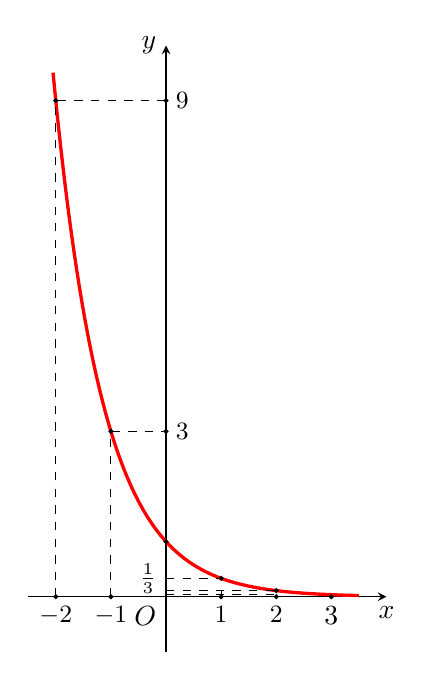
\begin{tikzpicture}[smooth,samples=100,scale=0.7,>=stealth]
					\draw[->] (-2.5,0)--(4,0) node[below]{$x$};
					\draw[->] (0,-1)--(0,10) node[left]{$y$};
					\draw (0,0) node[below left]{$O$};
					\draw[line width=1.2pt,color=red,domain=-2.05:3.5] plot(\x,{(1/3)^(\x)});
					\draw[fill=black] (0,1) circle(1pt) (0,3) circle(1pt) (0,9) circle(1pt)  (-2,0) circle(1pt) (-1,0) circle(1pt) (1,0) circle(1pt) (2,0) circle(1pt) (3,0) circle(1pt) node[below]{$3$} (-2,9) circle(1pt) (-1,3) circle(1pt) (1,1/3) circle(1pt) (2,1/9) circle(1pt);
					\draw[dashed] (-2,0)node[below]{\small $-2$}--(-2,9)--(0,9)node[right]{\small $9$};
					\draw[dashed] (-1,0)node[below]{\small $-1$}--(-1,3)--(0,3)node[right]{\small $3$};
					\draw[dashed] (0,1/3)node[left]{\small $\frac{1}{3}$}--(1,1/3)--(1,0)node[below]{\small $1$};
					\draw[dashed] (0,1/9)--(2,1/9)--(2,0)node[below]{\small $2$};
					\draw[dashed] (0,1/27)--(2,1/27);
					%\node[right] at (0,1) {$1$};
					%\node[below] at (0,-1.5) {$\text{Hình 6.2}$};
				\end{tikzpicture}
			}
	}
\end{bt}

\begin{bt}%[Tex hóa SGK CD-CT,T7/22, TVN-019]%[1T6B3-2]
	Vẽ đồ thị hàm số sau:
 $y=\left(\dfrac{1}{4}\right)^x$.
	\loigiai{ Lập bảng giá trị của hàm số ta được
			\begin{center}
				\begin{tabular}{|c|c|c|c|c|c|}
					\hline
					$x$ & $-1$ & $-\dfrac{1}{2}$ & $0$ & $\dfrac{1}{2}$ & $1$\\
					\hline
					$y=\left(\dfrac{1}{4}\right)^x$ & $4$ & $2$ & $1$ & $\dfrac{1}{2}$ & $\dfrac{1}{4}$\\
					\hline
				\end{tabular}
			\end{center}
			Đồ thị của hàm số $y=\left(\dfrac{1}{4}\right)^x$ như bên dưới
			\begin{center}
				\begin{tikzpicture}[>=stealth,line join=round,line cap=round,font=\footnotesize,scale=0.8]
					\draw[->] (-2,0)--(2,0) node[right] {$x$};
					\draw[->] (0,-1)--(0,4.8) node[above] {$y$};
					\draw [smooth,domain=-1.1:2,samples=100]plot(\x,{0.25^(\x)});
					\draw[dashed](-1,0)--(-1,4)--(0,4) (1,0)--(1,0.25)--(0,0.25);
					\fill (0,0)node[below right]{\footnotesize{$O$}}circle(1.2pt) (1,0)node[below]{\footnotesize{$1$}}circle(1.2pt) (-1,0)node[below]{\footnotesize{$-1$}}circle(1.2pt) (0,1)node[right]{\footnotesize{$1$}}circle(1.2pt) (0,4)node[right]{\footnotesize{$4$}}circle(1.2pt) (0,0.25)node[left]{\footnotesize{$\tfrac{1}{4}$}}circle(1.2pt) (1,0.25)circle(1.2pt) (-1,4)circle(1.2pt);
				\end{tikzpicture}
			\end{center}}
\end{bt}
\begin{bt}
	Vẽ đồ thị các hàm số sau
	\begin{enumerate}
		\item $y=\log_{\tfrac{1}{4}}x$.
		\item $y=\log_3 x$
	\end{enumerate}
	\loigiai{\begin{enumerate}
			\item Lập bảng giá trị của hàm số ta được
			\begin{center}
				\begin{tabular}{|c|c|c|c|c|c|}
					\hline
					$x$ & $\dfrac{1}{4}$ & $\dfrac{1}{2}$ & $1$ & $2$ & $4$ \\
					\hline
					$y=\log_{\tfrac{1}{4}}x$ & $1$ & $\dfrac{1}{2}$ & $0$ & $-\dfrac{1}{2}$ & $-1$\\
					\hline
				\end{tabular}
			\end{center}
			Đồ thị của hàm số $y=\log_{\tfrac{1}{4}}x$ như bên dưới
			\begin{center}
				\begin{tikzpicture}[>=stealth,line join=round,line cap=round,font=\footnotesize,scale=0.8]
					\draw[->] (-1,0)--(5,0) node[right] {$x$};
					\draw[->] (0,-2)--(0,2) node[above] {$y$};
					\draw [smooth,domain=0.065:5,samples=100]plot(\x,{(ln(\x))/(ln(0.25))});
					\draw[dashed](0.5,0)--(0.5,0.5)--(0,0.5) (4,0)--(4,-1)--(0,-1) (0.25,0)--(0.25,1)--(0,1);
					\fill (0,0)node[above left]{\footnotesize{$O$}}circle(1.2pt) (1,0)node[below]{\footnotesize{$1$}}circle(1.2pt) (4,0)node[above]{\footnotesize{$4$}}circle(1.2pt) (0.5,0)node[below]{\footnotesize{$\tfrac{1}{2}$}}circle(1.2pt) (0,1)node[left]{\footnotesize{$1$}}circle(1.2pt) (0,-1)node[left]{\footnotesize{$-1$}}circle(1.2pt) (0.5,0.5)circle(1.2pt) (4,-1)circle(1.2pt) (0.25,1)circle(1.2pt);
				\end{tikzpicture}
			\end{center}
			\item Vì hàm số $y=\log_3 x$ có cơ số $3>1$ nên ta có bảng biến thiên như sau
			\begin{center}
				
\begin{tikzpicture}[>=stealth,line join=round,line cap=round,font=\footnotesize,scale=1]
					\tkzTabInit[nocadre=false,lgt=2.3,espcl=2,deltacl=0.5]{$x$/0.7,$y=\log_3x$/2}
					{$0$ , $1$ , $+\infty$}
					\tkzTabVar{-/$-\infty$ , R , +/$+\infty$}
					\tkzTabIma{1}{3}{2}{$0$}% Từ cột 1 đến cột 3 đặt f(2) tại cột 2.
				\end{tikzpicture}
			\end{center}
			Đồ thị của hàm số $y=\log_3 x$ là một đường cong liền nét đi qua các điểm $A\left(\dfrac{1}{3};-1\right)$, $B(1;0)$, $C(3;1)$, $D(9;2)$.
			\begin{center}
				\begin{tikzpicture}[>=stealth,line join=round,line cap=round,font=\footnotesize,scale=0.9]
					\draw[->](-1,0) -- (10,0) node[below]{ $x$};
					\draw[->](0,-2) -- (0,4) node[below,right]{ $y$};
					\draw(-0.2,0) node[below left]{\footnotesize $O$};
					\clip(-1,-2) rectangle (10,4);
					\draw[smooth,samples=300,domain=0.1:9.5]plot(\x,{ln(\x)/ln(3)});
					\draw(1,0) node[below]{$1$}node[above]{$B$};
					\draw[dashed] (0,1) node[left]{$1$}--(3,1)node[above]{$C$}--(3,0)node[below]{$3$};
					\draw[dashed] (0,2) node[left]{$2$}--(9,2)node[above]{$D$}--(9,0)node[below]{$9$};
					\draw[dashed] (0,-1) node[left]{$-1$}--(1/3,-1)node[right]{$A$}--(1/3,0)node[above]{$\frac{1}{3}$};
					\draw (0.3,-1.6)node[right]{$y=\log_3x$};
				\end{tikzpicture}
			\end{center}
	\end{enumerate}}
\end{bt}
\begin{bt}
	So sánh các cặp số sau:
	\begin{enumEX}{2}
		\item $\log_{\pi}0{,}8$ và $\log_{\pi}1{,}2$.
		\item $\log_{0{,}3}2$ và $\log_{0{,}3}2{,}1$.
	\end{enumEX}
	\loigiai{\begin{enumerate}
			\item Hàm số $y=\log_{\pi}x$ có cơ số $\pi>1$ nên đồng biến trên $(0;+\infty)$.\\
			Mà $0{,}8<1{,}2$ nên $\log_{\pi}0{,}8<\log_{\pi}1{,}2$.
			\item Hàm số $y=\log_{0{,}3}x$ có cơ số $0{,}3<1$ nên nghịch biến trên $(0;+\infty)$.\\
			Mà $2<2{,}1$ nên $\log_{0{,}3}2>\log_{0{,}3}2{,}1$.
	\end{enumerate}}
\end{bt}
\begin{bt}%[Tex hóa SGK CD-CT,T7/22, TVN-019]%[1T6B3-3]
	So sánh các cặp số sau:
	\begin{enumEX}{2}
		\item $1{,}3^{0{,}7}$ và $1{,}3^{0{,}6}$.
		\item $0{,}75^{-2{,}3}$ và $0{,}75^{-2{,}4}$.
	\end{enumEX}
	\loigiai{\begin{enumerate}
			\item Do $1{,}3>1$ nên hàm số $y=1{,}3^x$ đồng biến trên $\mathbb{R}$. Mà $0{,}7>0{,}6$ nên $1{,}3^{0{,}7}>1{,}3^{0{,}6}$.
			\item Do $0{,}75<1$ nên hàm số $y=0{,}75^x$ nghịch biến trên $\mathbb{R}$. Mà $-2{,}3>-2{,}4$ nên $0{,}75^{-2{,}3}<0{,}75^{-2{,}4}$.
	\end{enumerate}}
\end{bt}
\subsubsection{Bài tập trắc nghiệm}

\Opensolutionfile{ans}[ans/ans-Bai3-Dang2]
\begin{ex}
	Hàm số nào dưới đây đồng biến trên tập xác định của nó?
	\choice
	{\True $y=\left(\sqrt{3}\right)^x $}
	{$ y=(0{,}6)^x $}
	{$ y = \left(\dfrac{\mathrm{e}}{5}\right)^x$}
	{ $y = \left(\dfrac{3}{4}\right)^x$ }
	\loigiai{
		Do $\sqrt{3} > 1$ nên hàm số $y = \left(\sqrt{3}\right)^x$ đồng biến trên $\mathbb{R}$.
	}
\end{ex}

\begin{ex}
	\immini{
		Hàm số nào sau đây có đồ thị như hình vẽ bên?
		\choice
		{\True $y=\left(\dfrac{1}{3}\right)^x$}
		{$y=(\sqrt{3})^x$}
		{$y=(\sqrt{2})^x$}
		{$y=\left(\dfrac{1}{2}\right)^x$}
	}{
		\begin{tikzpicture}[line cap=round,line join=round,>=stealth,font=\footnotesize,scale=1]
			\draw[->,color=black] (-2.,0.) -- (2.,0.);
			\foreach \x in {-1}
			\draw[shift={(\x,0)},color=black] (0pt,2pt) -- (0pt,-2pt) node[below] {$\x$};
			\draw[color=black] (1.68,-0.08) node [anchor=north west] {$x$};
			\draw[->,color=black] (0.,-0.5) -- (0.,4.);
			\foreach \y in {1,3}
			\draw[shift={(0,\y)},color=black] (2pt,0pt) -- (2pt,0pt) node[right] {$\y$};
			\draw[color=black] (0.1,3.8) node [anchor=west] {$y$};
			\draw[fill=black] (0,0)circle(1pt) node[below right] {$O$};
			\clip(-2.,-0.5) rectangle (2.,4.);
			\draw[smooth,samples=100,domain=-2.0:2.0] plot(\x,{(1.0/3.0)^((\x))});
			\draw [dash pattern=on 2pt off 2pt] (-1.,3.)-- (0.,3.);
			\draw [dash pattern=on 2pt off 2pt,fill=black] (-1.,3.)circle(1pt)-- (-1.,0.);
		\end{tikzpicture}
	}
	\loigiai{
		Đồ thị hàm số đi qua điểm $(-1;3)$, suy ra đây là đồ thị của hàm số $y=\left(\dfrac{1}{3}\right)^x$.
	}
\end{ex}


\begin{ex}
	Hàm số nào sau đây đồng biến trên khoảng $(-\infty;+\infty)$?
	\choice
	{$y=\left(\dfrac{\mathrm{e}}{4}\right)^x$}
	{$y=\left(\dfrac{2}{3}\right)^x$}
	{\True $y=\left(\dfrac{\pi}{3}\right)^x$}
	{$y=\left(\dfrac{3}{4}\right)^x$}
	\loigiai
	{Hàm số mũ $y=a^x$ đồng biến trên $(-\infty;+\infty)$ khi $a>1$.\\
		Vì $\dfrac{\pi}{3}>1$ nên hàm số $y=\left(\dfrac{\pi}{3}\right)^x$ đồng biến trên $(-\infty;+\infty)$.
	}
\end{ex}


\begin{ex}
	Hàm số nào sau đây đồng biến trên tập xác định của nó?
	\choice
	{$y=\left(\dfrac{3}{\pi}\right)^{x}$}
	{$y=\left(\sqrt{2020}-\sqrt{2019}\right)^{x}$}
	{$y=\log_{\tfrac{1}{2}} (x+4)$}
	{\True $y=\left(\dfrac{\sqrt{2}+\sqrt{3}}{\mathrm{e}}\right)^{x}$}
	\loigiai
	{
		Ta có $\sqrt{2}+\sqrt{3}>\mathrm{e}$ nên $\dfrac{\sqrt{2}+\sqrt{3}}{\mathrm{e}}>1$. \\
		Vậy hàm số $y=\left(\dfrac{\sqrt{2}+\sqrt{3}}{\mathrm{e}}\right)^{x}$ đồng biến trên tập xác định.
	}
\end{ex}

\begin{ex}
	Trong các hàm số sau, hàm số nào nghịch biến trên $\mathbb{R}$?
	\choice
	{$y=\left(\dfrac{2}{5}\right)^{-x}$}
	{\True $y=\left(\dfrac{\mathrm{e}}{4}\right)^{x}$}
	{$y=\log _{3} x^{2}$}
	{$y=\log \left(x^{3}\right)$}
	\loigiai{
		Ta có $0<\dfrac{\mathrm{e}}{4} <1$ do đó hàm số $y=\left(\dfrac{\mathrm{e}}{4}\right)^{x}$ nghịch biến trên $\mathbb{R}$.
	}
\end{ex}


\begin{ex}
	Trong các hàm số dưới đây, hàm số nào nghịch biến trên khoảng $\mathbb{R}$?
	\choice
	{\True $y=(0{,}5)^x$}
	{$y=2^x$}
	{$y=\pi^x$}
	{$y=\mathrm{e}^x$}
	\loigiai{
		Hàm số $y=a^x$ nghịch biến trên $\mathbb{R}$ khi và chỉ khi $0<a<1$.\\
		Vì $0<0{,}5<1$ nên hàm số $y=(0{,}5)^x$ nghịch biến trên $\mathbb{R}$.
	}
\end{ex}

\begin{ex}
	Cho hàm số $y=\mathrm{e}^x$. Mệnh đề nào sau đây là \textbf{sai}?
	\choice
	{\True Đồ thị hàm số đi qua điểm $A(1;0)$}
	{Tập xác định của hàm số $\mathscr{D}=\mathbb{R}$}
	{Hàm số có đạo hàm $y'=\mathrm{e}^x, \forall x \in \mathbb{R}$}
	{Đồ thị hàm số nhận trục hoành là tiệm cận ngang}
	\loigiai{
		Mệnh đề \textbf{sai} là \lq\lq Đồ thị hàm số đi qua điểm $A(1;0)$\rq\rq.
	}
\end{ex}

\begin{ex}
	Tìm tất cả các giá trị của $a$ để hàm số $y = (2020 - a)^x$ nghịch biến trên $\mathbb{R}$.
	\choice
	{$ a<2019$}
	{\True $2019 < a < 2020 $}
	{$ 0<a<1 $}
	{$ a<2020 $}
	\loigiai{
		Để hàm số $y = (2020 - a)^x$ nghịch biến trên $\mathbb{R}$ thì $0 < 2020 - a < 1 \Leftrightarrow 2019 < a < 2020$.	
	}
\end{ex}


\begin{ex}
	\immini{	Đồ thị trong hình vẽ bên dưới là đồ thị của hàm số nào sau đây?
		\choice
		{$y=(\sqrt{2})^x$}
		{$y=\left(\dfrac{1}{2}\right)^x $}
		{\True $\left( \dfrac{1}{3}\right)^x $}
		{$\left( \sqrt{3}\right)^x $}
	}{\begin{tikzpicture}[>=stealth,line join=round,line cap=round,font=\footnotesize,scale=.9]
			\draw[->](-1.5,0)--(3,0)node[scale=.9,below]{$x$};
			\draw[->](0,-.5)--(0,4)node[scale=.9,right]{$y$};
			\draw[domain=-1.2:3,samples=300] plot (\x,{(1/3)^(\x)});
			
			
			\fill (0,0)  circle (0.04) node[scale=0.9, below right]{$O$}
			(1,0)circle (0.04) node[scale=0.9, below]{$-1$}
			(0,1)circle (0.04) node[scale=0.9, above right]{$1$}
			(0,3)circle (0.04) node[scale=0.9,  right]{$3$}
			
			;
			\draw[dashed] (-1,0)|-(0,3)  
			;\
		\end{tikzpicture}
	}
	\loigiai
	{Đồ thị hàm số đi qua $(-1;3)$, do đó trong các đáp án đã cho thì đáp án thỏa mãn  là  $y=\left( \dfrac{1}{3}\right)^x $.
	}
\end{ex}

\begin{ex}
	Hàm số nào dưới đây nghịch biến trên tập xác định của nó?
	\choice
	{$y=(\sqrt{2})^x$}
	{$y=\left(\dfrac{3}{2}\right)^x$}
	{$y=\left(\dfrac{\pi}{\mathrm{e}}\right)^x$}
	{\True $y=(0{,}5)^x$}
	\loigiai{
		Hàm số $y=a^x$ có tập xác định $\mathscr{D}=\mathbb{R}$.
		\begin{itemize}
			\item Hàm số $y=a^x$ đồng biến trên $\mathbb{R}$ khi cơ số $a>1$.
			\item Hàm số $y=a^x$ nghịch biến trên $\mathbb{R}$ khi cơ số $0<a<1$.
		\end{itemize}
		Vậy $y=(0{,}5)^x$ nghịch biến trên tập xác định $\mathbb{R}$.
	}
\end{ex}


\begin{ex}
	Cho hai số thực $a, b$ khác $1$ và đồ thị của ba hàm số $y=a^{x}, y=b^{x}, y=2^{x}$ trên cùng một hệ trục tọa độ có dạng như hình vẽ bên.
	\begin{center}
		\begin{tikzpicture}[scale=0.9, font=\footnotesize, line join=round, line cap=round, >=stealth]
			\draw[->] (-3,0)--(0,0) node[below left]{$O$}--(4,0) node[below] {$x$};
			\draw[->] (0,-1)-- (0,5) node[left]{$y$};
			\draw[smooth,samples=100,domain=-2.5:2.5] plot(\x,{1/(1.8^(\x))}) node[above right]{$y=a^x$};
			\draw[smooth,samples=100,domain=-2.5:1.5] plot(\x,{2.5^(\x)}) node[above]{$y=b^x$};
			\draw[smooth,samples=100,domain=-2.5:2.5] plot(\x,{1.8^(\x)}) node[right]{$y=2^x$};
		\end{tikzpicture}
	\end{center}
	Mệnh đề nào sau đây đúng?
	\choice
	{$1<a<2, 1<b<2$}
	{$0<a<1, 1<b<2$}
	{\True $0<a<1, b>2$}
	{$1<a<2, b>2$}
	\loigiai{
		\immini
		{
			Quan sát đồ thị, ta thấy hàm số $y=a^x$ nghịch biến nên $0<a<1$.\\
			Kẻ đường thẳng $x=1$ cắt hai đồ thị hàm số $y=b^x$ và $y=2^x$ lần lượt tại hai điểm $A$ và $B$.\\
			Dễ thấy $y_A=b>y_B=2\Leftrightarrow b>2$.
		}
		{
			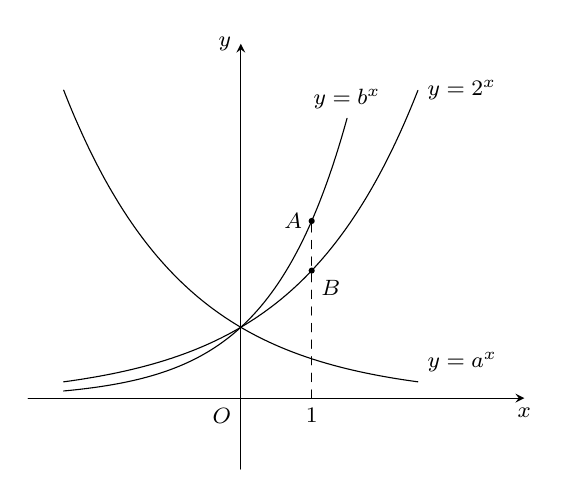
\begin{tikzpicture}[scale=0.9, font=\footnotesize, line join=round, line cap=round, >=stealth]
				\draw[->] (-3,0)--(0,0) node[below left]{$O$}--(4,0) node[below] {$x$};
				\draw[->] (0,-1)-- (0,5) node[left]{$y$};
				\draw[smooth,samples=100,domain=-2.5:2.5] plot(\x,{1/(1.8^(\x))}) node[above right]{$y=a^x$};
				\draw[smooth,samples=100,domain=-2.5:1.5] plot(\x,{2.5^(\x)}) node[above]{$y=b^x$};
				\draw[smooth,samples=100,domain=-2.5:2.5] plot(\x,{1.8^(\x)}) node[right]{$y=2^x$};
				\draw[fill=black] (1,0) node[below] {$1$} (1,2.5) node[left]{$A$} circle (1pt) (1,1.8) node[below right] {$B$} circle (1pt);
				
				\draw[dashed] (1,0)--(1,2.5);
			\end{tikzpicture}
		}
	}
\end{ex}
\begin{ex}
	\immini{	Cho đồ thị ba hàm số $ y=a^x $, $ y=b^x $, $ y=c^x $ như hình vẽ bên. Kết luận nào sau đây đúng?
		\choice
		{\True $0<c<1<b<a$}
		{$0<a<1<c<b$}
		{$0<a<1<b<c$}
		{$0<c<1<a<b$}}{
		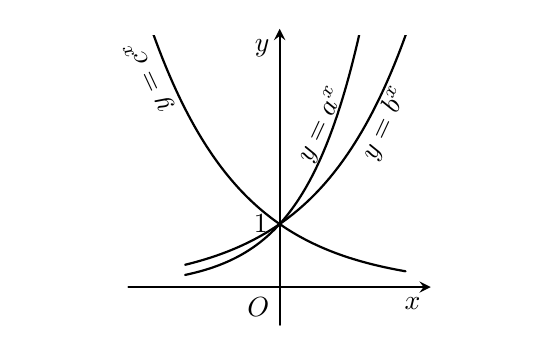
\begin{tikzpicture}[scale=0.8,line join=round, line cap=round,>=stealth,thick]
			\tikzset{label style/.style={font=\footnotesize}}
			\draw[->] (-2.4,0)--(2.4,0) node[below left] {$x$};
			\draw[->] (0,-0.6)--(0,4.1) node[below left] {$y$};
			\draw (0,0) node [below left] {$O$};
			\foreach \y in {1}
			\draw[thin] (1pt,\y)--(-1pt,\y) node [left] {$\y$};
			\begin{scope}
				\clip (-4,-0.5) rectangle (4,4);
				\draw[samples=200,domain=-3:2,smooth,variable=\x] plot (\x,{(1/2)^(\x)}) (-2.4,3.2) node[rotate =115,below]{$ y=c^x $};
				\draw[samples=200,domain=-1.5:2,smooth,variable=\x] plot (\x,{3^(\x)}) (1.0,3.3) node[rotate=65,left]{$ y=a^x $};
				\draw[samples=200,domain=-1.5:4,smooth,variable=\x] plot (\x,{2^(\x)}) (2,3.3) node[rotate=65,left]{$y= b^x $};
			\end{scope}
	\end{tikzpicture}}
	\loigiai{
		\begin{itemize}
			\item Đồ thị hàm số $ y=c^x  $ nghịch biến trên $ \mathbb{R} $, do đó $ 0<c<1 $.
			\item Đồ thị hàm số $ y=a^x  $, $ y=b^x $ đồng biến trên $ \mathbb{R} $, do đó $a>1$, $b>1 $.
			\item Với $ x=1 \Rightarrow a>b$.
		\end{itemize}
		Vậy $ a>b>1>c>0 $.
	}
\end{ex}
\begin{ex}
	Trong các hàm số sau đây, hàm số nào nghịch biến trên tập xác định của nó?
	\choice
	{$y=\ln x$}
	{$y=\log x$}
	{\True $y=\log _{\tfrac{2}{\mathrm{e}}}x$}
	{$y=\log _{\sqrt{3}}x$}
	\loigiai{
		Hàm số $y=\log _{\tfrac{2}{\mathrm{e}}}x$ có cơ số $a=\dfrac{\sqrt{2}}{\mathrm{e}}<1$ nên nghịch biến trên tập xác định.
	}
\end{ex}



\begin{ex}
	\immini{	Đường cong ở hình bên là đồ thị của một hàm số trong bốn hàm số được liệt kê ở bốn
		phương án  dưới đây. Hỏi hàm số đó là hàm số nào?.
		\choice
		{\True $y=\dfrac{1}{2^x}$}
		{$y=\log_{0{,}5}x$}
		{$y=2^x$}
		{$y=-x^2+2x+1$}}{\begin{tikzpicture}[xscale=1 ,yscale=0.7, line join=round, line cap=round,font=\footnotesize,>=stealth]
			\draw[fill,->] (-2.5,0)--(2.5,0) node [below] {$x$};
			\draw[->] (0,-1)--(0,4.5) node [left] {$y$};
			\draw[black,domain=-2.1:2.5]plot(\x,{(0.5)^(\x)});
			\draw[dashed] (-2,0)|-(0,4);
			\fill (0,1)node[above right]{$1$}
			(0,4)node[ right]{$4$}
			(-2,0)node[below]{$-2$}
			(0,0) node[below left]{$O$}circle(.03)
			
			
			;
	\end{tikzpicture}}
	\loigiai{
		Đồ thị hàm số hình bên đi qua điểm $(-2;4)$.\\
		Trong các đáp án chỉ có hàm số $y=\dfrac{1}{2^x}$ có đồ thị đi qua $(-2;4)$. Do đó $y=\dfrac{1}{2^x}$ là hàm số cần tìm.	
	}
\end{ex}


\begin{ex}
	\immini{Đường cong trong hình bên là đồ thị của một hàm số trong bốn hàm số được liệt kê ở bốn phương án $A$, $B$, $C$, $D$ dưới đây. Hỏi hàm số đó là hàm số nào?
		\choice
		{\True $y=\log_2x$}
		{$y=\log_{\sqrt{2}}x$}
		{$y=\log_2{2x}$}
		{$y=\log_{\tfrac{1}{2}}x$}}{	\begin{tikzpicture}[scale=1, font=\footnotesize,
			line join=round, line cap=round, >=stealth]
			\draw[->,line width = 1pt] (-2,0)--(0,0) node[below left]{$O$}--(4,0) node[below]{$x$};
			\draw[->,line width = 1pt] (0,-3.5) --(0,3) node[right]{$y$};
			\draw (0.5,0) node[above]{$\dfrac{1}{2}$} circle (1pt);
			\draw (1,0) node[below]{$1$} circle (1pt);
			\draw [thick,smooth,samples=290,domain=0.1:4] plot(\x,{ln(\x)/ln(2)});
			\draw [dashed] (0.5,0)--(0.5,-1)--(0,-1) node[left]{$-1$} circle(1pt);
	\end{tikzpicture}}
	
	\loigiai{
%		Dựa vào đồ thị ta thấy đồ thị hàm số đồng biến nên loại đáp án $y=\log_{\tfrac{1}{2}}x$.\\
		Ta thấy đồ thị hàm số đi qua điểm $A\left(\dfrac{1}{2};-1\right)$ nên thỏa mãn $y=\log_2x$.
	}
\end{ex}

\begin{ex}
	\immini{
		Tìm giá trị $a$ của hàm số $y=\log_{a}x$ ($0<a\neq 1$) có đồ thị như hình vẽ bên.
		\choice
		{\True $a=\sqrt{2}$}
		{$a=2$}
		{$a=\dfrac{1}{2}$}
		{$a=\dfrac{1}{\sqrt{2}}$}
	}{
		\begin{tikzpicture}[yscale=0.7,line join=round, line cap=round,>=stealth]
			\tikzset{label style/.style={font=\footnotesize}}
			\def\xmax{3}
			\def\xmin{-0.5}
			\def\ymax{3}
			\def\ymin{-1}
			\def\f(#1){ln(#1)/ln(sqrt(2))}
			\def\hamgoc{plot[domain=0.2:\xmax,smooth] (\x,{\f(\x)})}
			\begin{scope}
				\clip (\xmin,\ymin) rectangle (\xmax,\ymax);
				\draw[-stealth,name path=ox] (\xmin,0)--(\xmax,0) node[below left]{$x$};
				\draw[-stealth,name path=oy] (0,\ymin)--(0,\ymax) node[below right]{$y$};
				\draw[name path=dothi] \hamgoc;			
				\path (0,0) node[below left]{$O$}
				;
			\end{scope}
			\draw[dashed]
			(1,0)node[below]{$1$}
			(2,0)node[below]{$2$}|-(0,2)node[left]{$2$};
			\foreach \x/\y in {1/0,2/0,0/2}\fill (\x,\y) circle(1pt);
		\end{tikzpicture}
	}
	\loigiai{
		Ta thấy $\log_{a}2=2\Rightarrow a=\sqrt{2}$.	
	}
\end{ex}

\begin{ex}
	\immini{
		Đồ thị sau là của hàm số nào dưới đây?
		\choice
		{$y=\ln x$}
		{\True $y=2^x$}
		{$y=\log_2x$}
		{$y=4^x$}
	}{
		\begin{tikzpicture}[scale=.8,font=\footnotesize, line join=round,line cap=round,>=stealth]
			\draw[->] (-2,0)--(3,0)node[above]{$x$};
			\draw[->] (0,-1)--(0,5)node[left]{$y$};
			\draw[samples=100,domain=-2:2.3] plot(\x,{2^(\x)});
			\foreach \i/\j in {-1/-90,1/-90,2/-90}
			\draw[fill=black] (\i,0)node[shift=(\j:.32)]{$\i$}circle(1pt);
			\foreach \i/\j in {1/180,2/180,4/180}
			\draw[fill=black] (0,\i)node[shift=(\j:.32)]{$\i$}circle(1pt);
			\draw[fill=black] (0,0)node[below left]{$O$};
			\draw[dashed] (0,2)--(1,2)--(1,0);
		\end{tikzpicture}
	}
	\loigiai{
		Đồ thị hàm số luôn đi qua điểm $(0;1)$, suy ra đó là đồ thị của hàm số mũ.\\
		Quan sát thấy khi $x=1$ thì $y=2$, suy ra đó là đồ thị của hàm số $y=2^x$.
	}
\end{ex}


\begin{ex}
	Cho hàm số $y=\log_{\tfrac{1}{\sqrt{3}}}x$. Khẳng định nào dưới đây \textbf{sai}?
	\choice
	{Đồ thị hàm số đi qua điểm $(1;0)$}
	{\True Đồ thị hàm số nằm phía trên trục hoành}
	{Hàm số nghịch biến trên $(0;+\infty)$}
	{Đồ thị hàm số nằm bên phải trục tung}
	\loigiai{Đồ thị hàm số $y=\log_ax$ luôn cắt trục hoành tại điểm $(1;0)$, với mọi $a$ là số dương khác $1$.}
\end{ex}

\begin{ex}
	\immini{Đồ thị như hình vẽ bên là đồ thị của hàm số nào trong các hàm số sau
		\choice
		{$y=\log_\frac{3}{2}x$}
		{\True $y=\left(\dfrac{3}{2}\right)^x$}
		{$y=\left(\dfrac{1}{2}\right)^x$}
		{$y=\log_\frac{1}{2}x$}}
	{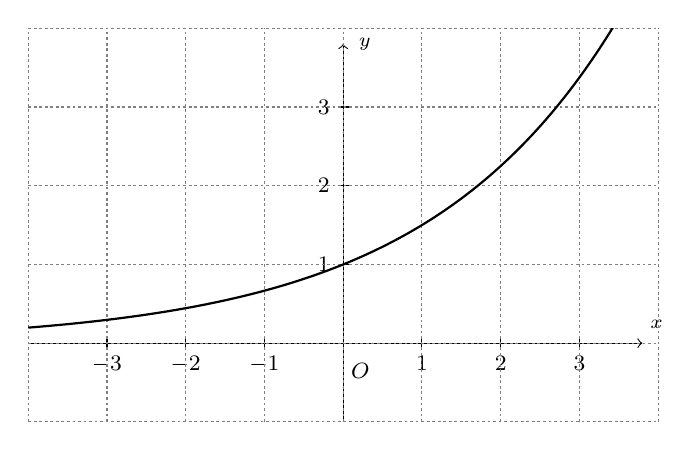
\begin{tikzpicture}%[>=stealth,scale=0.7]
			\begin{scriptsize}
				\draw[->] (-4,0.) -- (3.8,0.);
				\foreach \x in {-3,-2,-1,1,2,3}
				\draw[shift={(\x,0)}] (0pt,2pt) -- (0pt,-2pt) node[below] {\footnotesize $\x$};
				\draw (3.8,0.08) node [anchor=south west] {$x$};
				\draw[->] (0.,-1) -- (0.,3.8);
				\foreach \y in {1,2,3}
				\draw[shift={(0,\y)}] (2pt,0pt) -- (-2pt,0pt) node[left] {\footnotesize $\y$};
				\draw (0.1,3.8) node [anchor=west] {$y$};
				\draw [color=gray,dash pattern=on 1pt off 1pt, xstep=1.0cm,ystep=1.0cm] (-4,-1) grid (4,4);
				\draw (0pt,-10pt) node[right] {\footnotesize $O$};
			\end{scriptsize}
			\clip(-4,-1) rectangle (4,4);
			\draw[thick,smooth,samples=100,domain=-4:3.8] plot(\x,{
				(3/2)^(\x)});
	\end{tikzpicture}}
	\loigiai{
		Hàm số đồng biến do đó $a>1$.\\
		Đồ thị hàm số đi qua điểm $(0;1)$ nên là hàm số mũ $y=\left(\dfrac{3}{2}\right)^x$.
	}
\end{ex}

\begin{ex}
	\immini{Cho đồ thị hàm số $y=a^x, y= \log_b x$ (như hình vẽ). Khẳng định nào sau đây đúng?
		\choice
		{$0<b<1<a$}
		{\True $0<a<1<b$}
		{$a, b >1$}
		{$0<a, b<1$}
	}{
		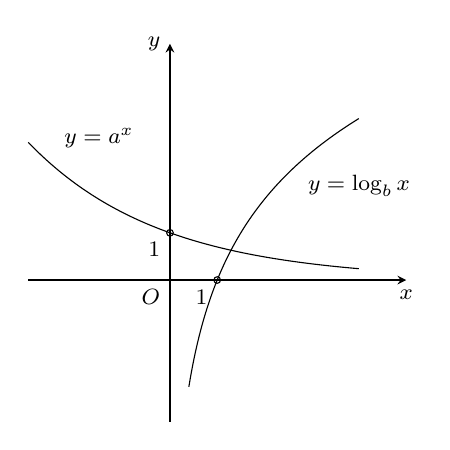
\begin{tikzpicture}[>=stealth,scale=0.6]
			\draw[->] (-3,0) -- (5,0) node[below] {\footnotesize $x$};
			\draw[->] (0,-3) -- (0,5) node[left] {\footnotesize $y$};
			\draw (0,0) node[below left] {\footnotesize $O$};
			\draw (0,1) node[below left] {\footnotesize $1$} circle (2pt);
			\draw (1,0) node[below left] {\footnotesize $1$} circle (2pt);
			\draw[line width=0.4pt,smooth,samples=200,domain=-3:4] plot(\x,{pow(0.7,\x)});
			\draw (-1.5,3) node {\footnotesize $y=a^x$};
			\draw[line width=0.4pt,smooth,samples=200,domain=0.4:4] plot(\x,{ln(\x)/ln(1.5)});
			\draw (4,2) node {\footnotesize $y= \log_b x$};
	\end{tikzpicture}}
	\loigiai{Đồ thị hàm số $y=a^x$ đi xuống nên $y=a^x$ nghịch biến. Suy ra $0<a<1$.\\
		Đồ thị hàm số $y= \log_b x$ đi lên nên $y= \log_b x$ đồng biến. Suy ra $b>1$.}
\end{ex}

\begin{ex}
	\immini
	{
		Cho hai hàm số $y=\log_ax$, $y=\log_bx$ với $a$, $b$ là hai số thực dương, khác $1$ có đồ thị lần lượt là $\left(C_1\right)$, $\left(C_2\right)$ như hình vẽ. Khẳng định nào sau đây \textbf{sai}?
		\choice
		{\True $0<b<a<1$}
		{$a>1$}
		{$0<b<1<a$}
		{$0<b<1$}
	}
	{
		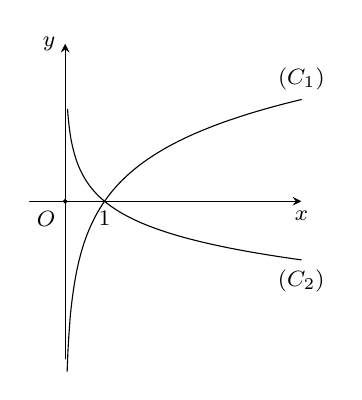
\begin{tikzpicture}[line join = round, line cap = round,>=stealth,font=\footnotesize,scale=0.5]
			\def\xp{6} \def\yt{4} \def\yd{-4} %x_phải, y_trên (giới hạn)
			%\draw[line width=0.1pt,dashed] (-0.9,\yd) grid (\xp,\yt); % Lưới toạ độ
			\draw[->] (-0.9,0)--(\xp,0) node [below]{$x$};
			\draw[->] (0,\yd)--(0,\yt) node [left]{$y$};
			\node at (0,0) [below left]{$O$};
			%\clip (-0.9,\yd) rectangle (\xp-0.1,\yt-0.1);
			\draw[smooth,samples=300,domain=0.05:\xp] plot(\x,{ln(\x)/ln(2)}) node[above]{$(C_1)$};
			\draw[smooth,samples=300,domain=0.06:\xp] plot(\x,{ln(\x)/ln(0.3)})node[below]{$(C_2)$};
			\draw (1,0) node[below]{$1$};
			\draw[fill=black] (0,0) circle(1.3pt);
		\end{tikzpicture} %câu 33
	}
	\loigiai{Ta thấy $\left(C_1\right)\colon y=\log_ax$ là hàm số đồng biến trên khoảng $(0;+\infty)$ suy ra $a>1$.\\
		Ta thấy $\left(C_2\right)\colon y=\log_bx$ là hàm số nghịch biến trên $(0;+\infty)$ suy ra $0<b<1$\\
		Vậy $0<b<1<a$. Do đó khẳng định $0<b<a<1$ sai.}
\end{ex}
\begin{ex}
	Cho $a$ là số thực dương khác $1$. Tìm mệnh đề đúng trong các mệnh đề sau.
	\choice
	{Đồ thị hàmg số $y=a^x$ với $0<a<1$ đồng biến trên khoảng $(-\infty;+\infty)$}
	{Hàm số $y=a^x$ với $a>1$ nghịch biến trên khoảng $(-\infty;+\infty)$}
	{Đồ thị hàm số $y=a^x$ luôn đi qua điểm $M(a;1)$}
	{\True Đồ thị hàm số $y=a^x$ và đồ thị hàm số $y=\log_ax$ đối xứng nhau qua đường thẳng $y=x$}
	\loigiai{
		Mệnh đề đúng là \lq\lq Đồ thị hàm số $y=a^x$ và đồ thị hàm số $y=\log_ax$ đối xứng nhau qua đường thẳng $y=x$ \rq\rq. Do nếu $M\left(m;a^m\right)$ thuộc đồ thị hàm số $y=a^x$ thì ta luôn suy ra điểm $N\left(a^m;m\right)$ thuộc đồ thị hàm số $y=\log_ax$.
		
	}
\end{ex}


\begin{ex}
	\immini{Cho đồ thị hàm số $y=a^x$, $y=\log_b x$ như hình vẽ. Trong các khẳng định sau, đâu là khẳng định đúng?
		\choice
		{\True $0<b<1<a$}
		{$a>1$, $b>1$}
		{$0<a<1<b$}
		{$0<a<1$, $0<b<1$}
	}
	{
		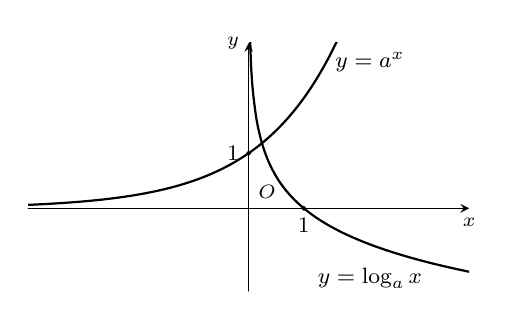
\begin{tikzpicture}[>=stealth,line cap=round,line join=round,scale=0.7,font=\footnotesize]
			\draw[->] (-4,0) -- (4,0) node[below] {\scriptsize $x$};
			\draw[->] (0,-1.5) -- (0,3) node[left] {\scriptsize $y$};
			\draw (0,0)node[above right]{\scriptsize $O$};
			\clip (-4,-1.5) rectangle(4,3);
			\draw[thick,samples=150,smooth,domain=-4:4] plot(\x,{2^(\x)});
			\draw[thick,samples=150,smooth,domain=0.01:4] plot(\x,{ln(\x)/ln(0.3)});
			\draw[fill=black] (0,1) circle(1pt) node[left]{$1$} (1,0) circle(1pt) node[below]{$1$} (2.2,3) node[below]{$y=a^x$} (2.2,-0.9) node[below]{$y=\log_a x$};
		\end{tikzpicture}	
	}
	\loigiai{
		Dựa vào đồ thị, ta thấy hàm số $y=a^x$ đồng biến trên $\mathbb{R}$ nên $a>1$, hàm số $y=\log_b x$ nghịch biến trên $(0;+\infty)$ nên $0<b<1$.\\
		Vậy $0<b<1<a$.
	}
\end{ex}

\begin{ex}
	\immini{
		Hàm số $ y=\log_ax\, \left(0<a\ne 1\right)$ có đồ thị là hình bên. Giá trị của cơ số $ a$ bằng
		\choice
		{$\sqrt[4]{2}$}
		{$ 4$}
		{\True $\sqrt{2}$}
		{$ 2$}
	}{
		\begin{tikzpicture}[scale=0.7, font=\footnotesize, line join=round, line cap=round, >=stealth]
			\tikzset{every node/.style={scale=0.9}}
			\draw[->] (-1.1,0)--(5.1,0) node[below] {$x$};
			\draw[->] (0,-2.1)--(0,5.1) node[left] {$y$};
			\fill[black](0,0) circle (1.3pt)($(0,0)+(-135:4mm)$) node{$O$};
			\foreach \x in {1,4}
			\draw[thin] (\x,1pt)--(\x,-1pt) node [below] {$\x$};
			\foreach \y in {4}
			\draw[thin] (1pt,\y)--(-1pt,\y) node [left] {$\y$};
			\draw[dashed, thin] (4,0)--(4,4)--(0,4);
			\begin{scope}
				\clip (-1,-2) rectangle (5,5);
				\draw[samples=200,domain=0.2:4.5,smooth,variable=\x] plot (\x,{ln((\x))/ln(sqrt(2))});
			\end{scope}
		\end{tikzpicture}
	}
	\loigiai{
		Từ đồ thị ta thấy, khi $x=4$ thì $y=4$. Điều này đúng khi $a=\sqrt{2}$.
	}
\end{ex}

\begin{ex}
	\immini
	{Đường cong trong hình bên dưới là đồ thị của một trong bốn hàm số được liệt kê ở bốn phương án A, B, C, D dưới đây. Hỏi hàm số đó là hàm số nào?
		\choice
		{$y=\log_2 x$}
		{$y=2^x$}
		{\True $y=\log_{\tfrac{1}{2}} x$}
		{$y=\left(\dfrac{1}{2}\right)^x$}}
	{
		\begin{tikzpicture}[line cap=round,line join=round,font=\footnotesize,>=stealth,scale=1]
			\draw[->] (-1,0)--(3,0) node[above] {$x$};
			\draw[->] (0,-1.5)--(0,2.5) node[left] {$y$};
			\fill (0,0) circle (1pt) node [below left] {$O$}
			(1,0) circle (1pt) node [above] {$1$}
			(2,0) circle (1pt) node [above] {$2$}
			(0,-1) circle (1pt) node [left] {$-1$}
			(2,-1) circle (1pt);
			\draw [samples=100, domain=0.2:2.8] plot (\x, {ln(\x)/ln(0.5)}); 
			\draw[dashed](2,0)|-(0,-1);
		\end{tikzpicture}
	}
	\loigiai
	{
		Dựa vào hình vẽ suy ra hàm số có dạng $y=\log_a x$ với cơ số $a<1$.\\
		Vậy hàm số thỏa mãn đề bài là $y=\log_{\tfrac{1}{2}} x$.
	}
\end{ex}
\begin{ex}
	\immini
	{
		Cho đồ thị các hàm số $ y=a^x $, $ y=b^x $ và $ y=\log_cx $ như hình vẽ. Khẳng định nào sau đây đúng?
		\choice
		{$b<a<c$}
		{\True $c<b<a$}
		{$c<a<b$}
		{$a<b<c$}
	}
	{
		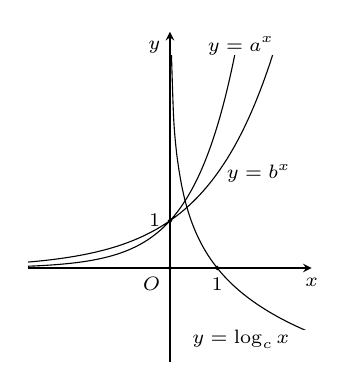
\begin{tikzpicture}[>=stealth,x=1cm,y=1cm,scale=0.6,font=\scriptsize] 
			\draw[->] (-3,0) -- (3,0) node[below] {$x$};
			\draw[->] (0,-2) -- (0,5) node[below left] {$y$};
			\draw[fill=black] (0,0) circle (1pt)node[below left] { $O$};
			\draw[fill=black] (1,0) circle (1pt)node[below] { $1$};
			\draw[fill=black] (0,1) circle (1pt)node[left] { $1$};
			\draw (1,2) node[right] { $y=b^x$} (1.5,-1.5) node { $y=\log_cx$} (1.5,4.7) node { $y=a^x$};
			\clip(-3,-1.3) rectangle (2.9,4.5);
			\draw[smooth,samples=100,domain=-3:3] plot(\x,{2^(\x)}) plot(\x,{3^(\x)});
			\draw[smooth,samples=100,domain=.02:5.5] plot(\x,{ln(\x)/ln(0.45)});
		\end{tikzpicture}
	}
	\loigiai
	{
		\begin{itemize}
			\item Vì hàm số $ y=\log_cx $ nghịch biến nên suy ra $ 0<c<1 $; hai hàm số $ y=a^x $, $ y=b^x $ đồng biến nên $ a, b>1 $.
			\item Với $ x=1 $, ta có $ a>b$.
		\end{itemize}
		Vậy $c<b<a$.
	}
\end{ex}

\begin{ex}
	\immini{Cho đồ thị của ba hàm số $y=\log _{a} x$, $y=\log _{b} x$,  $y=\log _{c} x$ như hình vē. Khẳng định nào sau đây đúng?
		\choice
		{$b>c>a$}
		{\True $b>a>c$}
		{$c>a>b$}
		{$c>b>a$}}{
		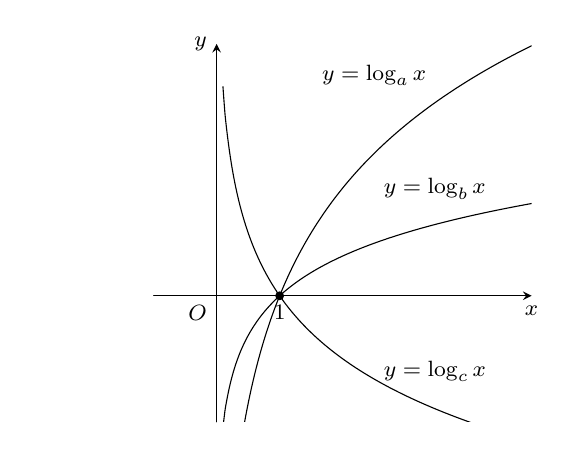
\begin{tikzpicture}[scale=0.8, font=\footnotesize, line join=round, line cap=round, >=stealth]
			\draw[->] (-1,0)--(5,0) node [below]{$x$};
			\draw[->] (0,-2)--(0,4) node [left]{$y$};
			\node at (0,0) [below left]{$O$};
			\clip (-3,-2) rectangle (5,4); 
			\fill[black] (1,0) circle (2pt) node [below] {$1$}  ;
			\draw[smooth,samples=150,domain=0.1:5] plot(\x,{ln(\x)/ln(3)});
			\draw[smooth,samples=150,domain=0.1:5] plot(\x,{ln(\x)/ln(1.5)});
			\draw[smooth,samples=150,domain=0.1:5] plot(\x,{ln(\x)/ln(0.5)});
			\node at (2.5,1.7)[right]{$y=\log_bx$};
			\node at (2.5,3.5){$y=\log_ax$};
			\node at (2.5,-1.2)[right]{$y=\log_cx$};
	\end{tikzpicture}}
	\loigiai{
		Quan sát đồ thị ta thấy 
		\begin{itemize}
			\item Cả hai đồ thị của hàm số $y=\log_a x$ và $y=\log_b x$ đều đi lên từ trái sang phải nên $a>1$ và $b>1$.
			\item Đồ thị của hàm số $y=\log_c x$ đi xuống từ trái sang phải nên $0<c<1$.
			\item Kẻ đường thẳng $y=1$ lần lượt cắt hai đồ thị $y=\log_a x$; $y=\log_b x$ tại hai điểm $A(a;1)$; $B(b;1)$. Suy ra $ a< b$.\\
			Vậy $b>a>c$.
		\end{itemize}
	}
\end{ex}
\Closesolutionfile{ans}
\begin{indapan}{10}
	{ans/ans-Bai3-Dang2}
\end{indapan}

\begin{dang}{Bài toán thực tế}
\end{dang}
\subsubsection{Ví dụ mẫu}

\begin{vd}%[CD]%[Đỗ Minh Phúc]%[1C6B3-4]
	Ta coi năm lấy làm mốc để tính dân số của một vùng (hoặc một quốc gia) là năm 0. Khi đó, dân số của quốc gia đó ở năm thứ $t$ là hàm số theo biến $t$ được cho bởi công thức: $S=A \cdot \mathrm{e}^{rt}$. Trong đó $A$ là dân số của vùng (hoặc quốc gia) đó ở năm 0 và $r$ là tỉ lệ tăng dân số hằng năm (Nguồn: Giải tích 12, NXBGD Việt Nam, 2021). Biết rằng dân số Việt Nam năm 2021 ước tính là $98564407$ người và tỉ lệ tăng dân số $0,93\%$/năm (Nguồn: https://danso.org/viet-nam). Giả sử tỉ lệ tăng dân số hằng năm là như nhau tính từ năm 2021, nêu dự đoán dân số Việt Nam năm 2030 (làm tròn kết quả đến hàng đơn vị).
	\loigiai{
		Dân số Việt Nam vào năm 2030 là
		$$S=A \cdot \mathrm{e}^{rt}=98564407\cdot \mathrm{e}^{0,93\%\cdot 9}\approx 107169341\text{ (người).}$$
	}
\end{vd}
\begin{vd} %[Tex hóa SGK CD-CT,T7/22, TVN-019]%[1T6B3-4]
	Năm 2020, dân số thế giới là $7{,}795$ tỉ người và tốc độ tăng dân số là $1{,}05$\%/năm (nguồn: http://www.worldmeters.info/world-population). Nếu tốc độ tăng này tiếp tục duy trì ở những năm tiếp theo thì dân số thế giới sau $t$ năm kể từ năm 2020 được tính bởi công thức
	$$P(t)=7{,}795\cdot(1+0{,}0105)^t\text{ (tỉ người).}\qquad(*)$$
	Khi đó, hãy tính dân số thế giới vào năm 2025 và năm 2030. (Mốc thời điểm để tính dân số của mỗi năm là ngày 1 tháng 7.)
	\loigiai{Năm 2025 ứng với $t=5$ nên có dân số thế giới là
		$$P(5)=7{,}795\cdot(1+0{,}0105)^5\approx8{,}213\text{ (tỉ người).}$$
		Năm 2030 ứng với $t=10$ nên có dân số thế giới là
		$$P(10)=7{,}795\cdot(1+0{,}0105)^{10}\approx8{,}653\text{ (tỉ người).}$$}
\end{vd}
\textbf{Chú ý:} Với giả thiết tốc độ tăng dân số $1{,}05$\%/năm không đổi, công thức $(*)$ được áp dụng để tính dân số thế giới tại thời điểm bất kì sau năm 2020. Chẳng hạn, dân số thế giới tại thời điểm ngày 1 tháng 1 năm 2022 (ứng với $t=1{,}5$) là 
$$P(1{,}5)=7{,}795\cdot(1+0{,}0105)^{1{,}5}\approx7{,}918\text{ (tỉ người).}$$


\begin{vd}%[CD]%[Đỗ Minh Phúc]%[1C6B3-4]
	Trong Vật lí, sự phân rã của các chất phóng xạ được cho bởi công thức: $m(t)=m_0 \cdot\left(\dfrac{1}{2}\right)^{\tfrac{t}{T}} ;$ trong đó $m_0$ là khối lượng chất phóng xạ ban đầu (tại thời điểm $t=0$ ), $m(t)$ là khối lượng chất phóng xạ tại thời điểm $t$ và $T$ là chu kì bán rã (Nguồn: Giải tích 12, NXBGD Việt Nam, 2021). Hạt nhân Poloni (Po) là chất phóng xạ $\alpha$ có chu kì bán rã là $138$ ngày (Nguồn: Vật lí 12, NXBGD Việt Nam, 2021). Giả sử lúc đầu có $100$ gam Poloni. Tính khối lượng Poloni còn lại sau $100$ ngày theo đơn vị gam (làm tròn kết quả đến hàng phần mười).
	\loigiai{
		Khối lượng Poloni còn lại sau $100$ ngày là
		$$m(100)=100 \cdot\left(\dfrac{1}{2}\right)^{\tfrac{100}{138}} \approx 60,5(\mathrm{~g}).$$}
\end{vd}

\begin{vd}%[CD]%[Đỗ Minh Phúc]%[1C6B3-4]
	Lốc xoáy là hiện tượng một luồng không khí xoáy tròn mở rộng ra từ một đám mây dông xuống tới mặt đất. Các cơn lốc xoáy thường có sức tàn phá rất lớn. Tốc độ của gió (đơn vị: dặm/giờ) gần tâm của một cơn lốc xoáy được tính bởi công thức: $S=93 \log d+65$, (Nguồn: Ron Larson, Intermediate Algebra, Cengage) trong đó $d$ (đơn vị: dặm) là quãng đường cơn lốc xoáy di chuyển được. Hãy tính tốc độ của gió ở gần tâm (làm tròn kết quả đến hàng đơn vị) khi cơn lốc xoáy di chuyển được quãng đường là
	\begin{multicols}{2}
		\begin{enumerate}
			\item $5$ dặm
			\item $10$ dặm
		\end{enumerate}
	\end{multicols}
	\loigiai{
		\begin{enumerate}
			\item Tốc độ của gió ở gần tâm khi cơn lốc xoáy di chuyển được quãng đường $5$ dặm là
			$$S=93 \log 5+65 \approx 130 \text { (dặm/giờ).}$$
			\item Tốc độ của gió ở gần tâm khi cơn lốc xoáy di chuyển được quãng đường $10$ dặm là
			$$S=93 \log 10+65=158\text { (dặm/giờ)}.$$
		\end{enumerate}
	}
\end{vd}
\begin{vd} %[Tex hóa SGK CD-CT,T7/22, TVN-019]%[1T6B3-4]
	Trong âm học, mức cường độ âm được tính bới công thức $L=10\log\left(\dfrac{I}{I_0}\right)$ (dB) (dB là đơn vị mức cường độ âm, đọc là đề-xi-ben), trong đó $I$ là cường độ âm tính theo W/m$^2$ và $I_0=10^{-12}$ W/m$^2$ là cường độ âm chuẩn (cường độ âm thấp nhất mà tai người bình thường có thể nghe được).
	\begin{center}
		(\textit{Nguồn:} Vật lí 12, NXB Giáo dục Việt Nam, năm 2017, trang 52,53)
	\end{center}
	\begin{enumerate}
		\item Mức cường độ âm $L$ thấp nhất mà tai người có thể nghe được là bao nhiêu?
		\item Cuộc trò chuyện có cường độ âm $10^{-9}$ W/m$^2$ thì có mức cường độ âm bằng bao nhiêu?
		\item Cường độ âm tại một khu văn phòng nằm trong miền từ $10^{-7}$ W/m$^2$ đến $5\cdot10^{-6}$ W/m$^2$ (tức là $10^{-7}\le I\le5\cdot10^{-6}$). Mức cường độ âm tại khu văn phòng này nằm trong khoảng nào? (Làm tròn kết quả đến hàng đơn vị).
	\end{enumerate}
	\loigiai{\begin{enumerate}
			\item Khi $I=I_0$ thì $L=10\log 1=0$ (dB). Vậy mức cường độ âm thấp nhất mà tai người bình thường có thể nghe được là $0$ (dB).
			\item Khi $I=10^{-9}$ W/m$^2$, ta có $L=10\log\dfrac{10^{-9}}{10^{-12}}=10\log10^3=30\log10=30$ (dB).
			\item Với $I=10^{-7}$ W/m$^2$, $L=10\log\dfrac{10^{-7}}{10^{-12}}=10\log10^5=50\log10=50$ (dB).\\
			Với $I=5\cdot10^{-6}$ W/m$^2$, $L=10\log\dfrac{5\cdot10^{-6}}{10^{-12}}=10\log\left(5\cdot10^6\right)=10(6+\log5)\approx67$ (dB).\\
			Hàm số $y=\log x$ đồng biến nên hàm số $y=10\log x$ cũng đồng biến.\\
			Do đó, từ $10^{-7}\le I\le5\cdot10^{-6}$ suy ra $50\le L\le67$.\\
			Vậy mức cường độ âm tại khu văn phòng nằm trong khoảng từ $50$ (dB) đến $67$ (dB).
	\end{enumerate}}
\end{vd}


\subsubsection{Bài tập rèn luyện }

\begin{bt}%[Tex hóa SGK CD-CT,T7/22, TVN-001]%[1K6YI-4]
	Giả sử một chất phóng xạ bị phân rã theo cách sao cho khối lượng $m(t)$ của chất còn lại (tính bằng kilôgam) sau $t$ ngày được cho bởi hàm số $m(t) = 13 \mathrm{e}^{-0,0015t}$.
	\begin{enumerate}
		\item Tìm khối lượng của chất đó tại thời điểm $t = 0$.
		\item Sau 45 ngày khối lượng chất đó còn lại là bao nhiêu?
	\end{enumerate}
	\loigiai{
		\begin{enumerate}
			\item $m(0) = 13\mathrm e^{0} = 13$ (kilôgam).
			\item $m(45) = 13\mathrm e^{-0,015 \cdot  45} \approx 6{,}62$ (kilôgam).
		\end{enumerate}
	}
\end{bt}

\begin{bt}%[Đỗ Minh Phúc]%[1C6B3-4]
	Các nhà tâm lí học sử dụng mô hình hàm số mũ để mô phỏng quá trình học tập của một học sinh như sau: $f(t)=c\left(1-e^{-k t}\right)$, trong đó $c$ là tổng số đơn vị kiến thức học sinh phải học, $k$ (kiến thức/ngày) là tốc độ tiếp thu của học sinh, $t$ (ngày) là thời gian học và $f(t)$ là số đơn vị kiến thức học sinh đã học được (Nguồn: R.I. Charles et al., Algebra 2, Pearson). Giả sử một em học sinh phải tiếp thu $25$ đơn vị kiến thức mới. Biết rằng tốc độ tiếp thu của em học $\sinh$ là $k=0{,}2$. Hỏi em học sinh sẽ nhớ được (khoảng) bao nhiêu đơn vị kiến thức mới sau $2$ ngày? Sau $8$ ngày?
	\loigiai{
		Số đơn vị kiến thức mới em học sinh sẽ nhớ sau $2$ ngày là
		$$f(2)=25\left(1-e^{-0{,}2\cdot2}\right)\approx 8{,}24\text{ (đơn vị)}.$$
		Số đơn vị kiến thức mới em học sinh sẽ nhớ sau $8$ ngày là
		$$f(8)=25\left(1-e^{-0{,}2\cdot8}\right)\approx 19{,}95\text{ (đơn vị)}.$$
	}	
\end{bt}

\begin{bt}
	Chỉ số hay độ pH của một dung dịch được tính theo công thức: $\mathrm{pH}=-\log \left[\mathrm{H}^{+}\right]$. Phân tích nồng độ ion hydrogen $\left[\mathrm{H}^{+}\right]$ trong hai mẫu nước sông, ta có kết quả sau: Mẫu 1: $\left[\mathrm{H}^{+}\right]=8 \cdot 10^{-7}$; Mẫu $2:\left[\mathrm{H}^{+}\right]=2 \cdot 10^{-9}$.
	Không dùng máy tính cầm tay, hãy so sánh độ pH của hai mẫu nước trên.
	\loigiai{
		Hàm số $\mathrm{pH}=-\log \left[\mathrm{H}^{+}\right]$ có $a=10>1$ nên nghịch biến trên $(0;+\infty)$.\\
		Vì $8 \cdot 10^{-7}>2 \cdot 10^{-9}$ nên độ pH của mẫu 1 bé hơn độ pH của mẫu 2.
	}
\end{bt}
\begin{bt}%[Tex hóa SGK CD-CT,T7/22, TVN-019]%[1T6B3-4]
	Cường độ ánh sáng $I$ dưới mặt biển giảm dần theo độ sâu theo công thức $I=I_0\cdot a^d$, trong đó $I_0$ là cường độ ánh sáng tại mặt nước biển, $a>0$ là hằng số và $d$ là độ sâu tính bằng mét tính từ mặt nước biển.
	\begin{center}
		(\textit{Nguồn:}  http://www.britannica.com/science/seawer/Optical-properties)
	\end{center}
	\begin{enumerate}
		\item Có thể khẳng định rằng $0<a<1$ không? Giải thích.
		\item Biết rằng cường độ ánh sáng tại độ sâu $1$m bằng $0{,}95I_0$. Tìm giá trị của $a$.
		\item Tại độ sâu $20$m, cường độ ánh sáng bằng bao nhiêu phần trăm so với $I_0$? (Làm tròn kết quả đến hàng đơn vị.)
	\end{enumerate}
	\loigiai{\begin{enumerate}
			\item Do $I_0$ là cường độ ánh sáng tại mặt nước biển là không đổi, nên cường độ ánh sáng $I$ tỉ lệ thuận với hàm số $a^d$.\\
			Do $I$ giảm dần theo độ sâu, nên hàm số $a^d$ nghịch biến, suy ra $0<a<1$.
			\item Tại độ sâu $1$m, ta có cường độ ánh sáng $I=0{,}95I_0$, suy ra $0{,}95I_0=I_0a^1\Leftrightarrow a=0{,}95$.
			\item Tại độ sâu $20$m, suy ra $d=20$. Cường độ ánh sáng tại đó là $I=I_0a^d=I_0\cdot0{,}95^{20}\approx0{,}4I_0$.\\
			Vậy tại độ sâu $20$m, cường độ ánh sáng tại đó bằng khoảng $40$\% so với $I_0$.
	\end{enumerate}}
\end{bt}
\begin{bt}
	Một người gửi $10$ triệu đồng vào ngân hàng theo hình thức lãi kép có kì hạn là 12 tháng vối lãi suất $6\%$/năm. Giả sử qua các năm thì lãi suất không thay đổi và người đó không gửi thêm tiền vào mỗi năm. Để biết sau $y$ (năm) thì tổng số tiền cả vốn và lãi có được là $x$ (đồng), người đó sử dụng công thức $y=\log_{1,06}\left(\dfrac{x}{10}\right)$. Hỏi sau bao nhiêu năm thì người đó có được tổng số tiền cả vốn và lãi là $15$ triệu đồng? $20$ triệu đồng? (Làm tròn kết quả đến hàng đơn vị).
	\loigiai{
		Người đó có được tổng số tiền cả vốn lẫn lãi là $15$ triệu đồng sau
		$$y=\log_{1,06}\left(\dfrac{15}{10}\right)\approx 7\text{ (năm).}$$
		Người đó có được tổng số tiền cả vốn lẫn lãi là $20$ triệu đồng sau
		$$y=\log_{1,06}\left(\dfrac{20}{10}\right)\approx 12\text{ (năm).}$$
	}
\end{bt}
\begin{bt}
	Trong một nghiên cứu, một nhóm học sinh được cho xem cùng một danh sách các loài động vật và được kiểm tra lại xem họ còn nhớ bao nhiêu phần trăm danh sách đó sau mỗi tháng. Giả sử sau $t$ tháng, khả năng nhớ trung bình của nhóm học sinh đó được tính theo công thức $M(t) = 75 - 20 \ln (t+1), \enskip 0 \leq t \leq 12$ (đơn vị: \%). Hãy tính khả năng nhớ trung bình của nhóm học sinh đó sau 6 tháng.
	\loigiai{
		Khả năng nhớ trung bình của nhóm học sinh đó sau 6 tháng là $$M(6) = 75 - 20 \ln (6+1) \approx 36{,}1 \%.$$
	}
\end{bt}
\begin{bt}
	Cường độ ánh sáng $I$ dưới mặt biển giảm dần theo độ sâu theo công thức $I=I_0\cdot a^d$, trong đó $I_0$ là cường độ ánh sáng tại mặt nước biển, $a>0$ là hằng số và $d$ là độ sâu tính bằng mét tính từ mặt nước biển.
	\begin{center}
		(\textit{Nguồn:}  http://www.britannica.com/science/seawer/Optical-properties)
	\end{center}
	\begin{enumerate}
		\item Có thể khẳng định rằng $0<a<1$ không? Giải thích.
		\item Biết rằng cường độ ánh sáng tại độ sâu $1$m bằng $0{,}95I_0$. Tìm giá trị của $a$.
		\item Tại độ sâu $20$m, cường độ ánh sáng bằng bao nhiêu phần trăm so với $I_0$? (Làm tròn kết quả đến hàng đơn vị.)
	\end{enumerate}
	\loigiai{\begin{enumerate}
			\item Do $I_0$ là cường độ ánh sáng tại mặt nước biển là không đổi, nên cường độ ánh sáng $I$ tỉ lệ thuận với hàm số $a^d$.\\
			Do $I$ giảm dần theo độ sâu, nên hàm số $a^d$ nghịch biến, suy ra $0<a<1$.
			\item Tại độ sâu $1$m, ta có cường độ ánh sáng $I=0{,}95I_0$, suy ra $0{,}95I_0=I_0a^1\Leftrightarrow a=0{,}95$.
			\item Tại độ sâu $20$m, suy ra $d=20$. Cường độ ánh sáng tại đó là $I=I_0a^d=I_0\cdot0{,}95^{20}\approx0{,}4I_0$.\\
			Vậy tại độ sâu $20$m, cường độ ánh sáng tại đó bằng khoảng $40$\% so với $I_0$.
	\end{enumerate}}
\end{bt}
\begin{bt}
	Công thức $h=-19{,}4\cdot\log\dfrac{P}{P_0}$ là mô hình đơn giản cho phép tính độ cao $h$ so với mặt nước biển của một vị trí trong không trung (tính bằng ki-lô-mét) theo áp suất không khí $P$ tại điểm đó và áp suất $P_0$ của không khí tại mặt nước biển (cùng tính bằng $Pa$ - đơn vị áp suất, đọc là Pascal).
	\begin{center}
		(\textit{Nguồn:}  http://doi.org/10.1007/s40828-020-0111-6)
	\end{center}
	\begin{enumerate}
		\item Nếu áp suất không khí ngoài máy bay bằng $\dfrac{1}{2}P_0$ thì máy bay đang ở độ cao nào?
		\item Áp suất không khí tại đỉnh của ngọn núi A bằng $\dfrac{4}{5}$ lần áp suất không khí tại đỉnh của ngọn núi B. Ngọn núi nào cao hơn và cao hơn bao nhiêu ki-lô-mét? (Làm tròn kết quả đến hàng phần mười.)
	\end{enumerate}
	\loigiai{\begin{enumerate}
			\item Nếu áp suất ở ngoài máy bay là $\dfrac{1}{2}P_0$ thì độ cao của máy bay là $$h=-19{,}4\cdot\log\dfrac{\dfrac{1}{2}P_0}{P_0}=-19{,}4\cdot\log\dfrac{1}{2}\approx5{,}8\text{km}.$$
			\item Gọi áp suất lần lượt của hai ngọn núi A và B là $P_A$, $P_B$. Ta có $P_A=\dfrac{4}{5}P_B$.\\
			Độ cao của núi A và núi B là $\heva{&h_A=-19{,}4\cdot\log\dfrac{P_A}{P_0}\\&h_B=-19{,}4\cdot\log\dfrac{P_B}{P_0}.}$\\
			Ta có
			\begin{eqnarray*}
				h_A&=&-19{,}4\cdot\log\dfrac{P_A}{P_0}=-19{,}4\cdot\log\dfrac{\dfrac{4}{5}P_B}{P_0}\\
				&=&-19{,}4\cdot\left(\log\dfrac{4}{5}+\log\dfrac{P_B}{P_0}\right)=-19{,}4\cdot\log\dfrac{4}{5}+h_B\approx h_B+1{,}9.
			\end{eqnarray*}
			Vậy núi A cao hơn núi B $1{,}9$km.
	\end{enumerate}}
\end{bt}

\subsubsection{Bài tập trắc nghiệm}

\Opensolutionfile{ans}[ans/ans-Bai3-Dang3]
\begin{ex}
	Một quần thể vi khuẩn bắt đầu từ $100$ cá thể và cứ sau $3$ giờ thì số cá thể lại tăng gấp đôi. Bởi vậy số cá thể vi khuẩn được biểu thị theo thời gian $t$ (đơn vị giờ) bằng công thức $N(t)=100\cdot 2^{\frac{t}{3}}$. Hỏi sau bao lâu thì quần thể này đạt tới $50000$ cá thể (làm tròn đến hàng phần mười)?	
	\choice
	{$36{,}8$ giờ}
	{$30{,}2$ giờ}
	{\True $26{,}9$ giờ}
	{$18{,}6$ giờ}
	\loigiai{
		Ta có $100\cdot2^{\frac{t}{3}}=50000 \Leftrightarrow 2^{\frac{t}{3}}=500 \Leftrightarrow t=3\cdot \log _2 500 \Rightarrow t \approx 26{,}9$.
	}
\end{ex}
\begin{ex}
	Năm $2020$, một doanh nghiệp X có tổng doanh thu là $150$ tỉ đồng. Dự kiến trong $10$ năm tiếp theo, tổng doanh thu mỗi năm sẽ tăng thêm $12$\% so với năm liền trước. Theo dự kiến đó thì kể từ năm nào, tổng doanh thu của doanh nghiệp X vượt quá $360$ tỉ đồng?
	\choice
	{$2026$}
	{$2027$}
	{\True $2028$}
	{$2029$}
	\loigiai
	{
		Do mỗi năm doanh thu tăng thêm $12$\% nên tổng doanh thu sau $n$ năm là $P_n=P(1+r)^n$, trong đó $P$ là số doanh thu ban đầu, $r$ là số phần trăm tăng thêm hằng năm.\\
		Theo đề bài ta có
		\[P(1+r)^n>360\Leftrightarrow 150(1+12\%)^n>360\Leftrightarrow n>\log_{1{,}12}2{,4}\approx7{,}73.\]
		Vậy kể từ năm $2028$, tổng doanh thu của doanh nghiệp X vượt quá $360$ tỉ đồng.
	}
\end{ex}

\begin{ex}
	Một người gửi tiền vào ngân hàng với lãi suất không thay đổi là $6\%$/ năm. Biết rằng nếu không rút tiền ra khỏi ngân hàng thì cứ sau mỗi năm, số tiền lãi sẽ được nhập vào vốn ban đầu (người ta gọi là lãi kép). Người đó định gửi tiền trong vòng $3$ năm, sau đó rút ra $500$ triệu đồng. Hỏi số tiền ít nhất người đó phải gửi trong ngân hàng (làm tròn đến hàng triệu) là bao nhiêu triệu đồng?
	\choice
	{\True $420$}
	{$410$}
	{$400$}
	{$390$}
	\loigiai{
		Gọi $A$ là số tiền ban đầu cần gửi, $r=0{,}06$ là lãi suất hàng năm.\\
		Sau $3$ năm, số tiền cả gốc lẫn lãi của người đó là 
		$S=A(1+r)^3$.\\
		Ta có $S\ge 500\Leftrightarrow A(1+r)^3\ge 500\Leftrightarrow A\ge \dfrac{500}{(1+r)^3}=\dfrac{500}{1{,06}^3}\approx 420$ triệu.
	}
\end{ex}

\begin{ex}
	Ông Hùng dự định gửi vào ngân hàng một số tiền với lãi suất $6{,}5\%$ một năm. Biết rằng cứ sau mỗi năm số tiền lãi sẽ gộp vào vốn ban đầu. Số tiền $x$ (triệu đồng, $x\in\mathbb{N}$) nhỏ nhất mà ông Hùng cần gửi vào ngân hàng để sau ba năm (mới rút lãi) thì số tiền lãi có thể mua một chiếc xe máy trị giá $60$ triệu đồng là
	\choice
	{$280$}
	{\True $289$}
	{$300$}
	{$308$}
	\loigiai{
		Số tiền thu được sau ba năm (cả tiền lãi và tiền gốc) là $x(1+6{,}5\%)^3$.\\
		Ta có $x(1+6{,}5\%)^3-x=60\Rightarrow x\approx 289$ triệu đồng.}
\end{ex}


\begin{ex}
	Ông X gửi vào ngân hàng $60$ triệu đồng theo hình thức lãi kép. Lãi suất ngân hàng là  $8\%$ trên năm. Sau $5$ năm ông X tiếp tục gửi thêm $60$ triệu đồng nữa. Hỏi sau $10$ năm kể từ lần gửi đầu tiên ông X đến rút toàn bộ tiền gốc và tiền lãi được là bao nhiêu? (Biết lãi suất không thay đổi qua các năm ông X gửi tiền).
	\choice
	{\True $217{,}695$ (triệu đồng)}
	{$231{,}815$ (triệu đồng)}
	{$190{,}271$ (triệu đồng)}
	{$197{,}201$ (triệu đồng)}
	\loigiai
	{Công thức tính tiền gốc lẫn lãi của hình thức gửi ngân hàng theo lãi kép là $T_n=A(1+r)^n$, trong đó $A$ là số tiền gửi ban đầu, $r$ là lãi suất hàng năm, $n$ là số năm gửi.\\
		Vậy tổng số tiền ông X nhận được là $$60\cdot (1+0.08)^{10}+60\cdot (1+0.08)^5\approx 217{,}695\ (\text{triệu đồng}).$$
	}
\end{ex}

\begin{ex}
	Năm $2000$ và năm $2020$, giá xăng trung bình ở Việt Nam lần lượt là $5000$ VNĐ/ $1$ lít và $15000$ VNĐ/ $1$ lít. Giả sử $r\%$ là tỷ lệ tăng giá xăng trung bình hàng năm trong giai đoạn từ năm $2000$ đến năm $2020$ ở Việt Nam. Hỏi $r\%$ bằng bao nhiêu?
	\choice
	{$5{,}46\%$}
	{$5\%$}
	{$4{,}56\%$}
	{\True $5{,}64\%$}
	\loigiai
	{
		Từ năm $2000$ đến năm $2020$ có tổng thời gian là $20$ năm.\\
		Theo đề bài ta có phương trình
		\[15000=5000(1+r)^{20}\Leftrightarrow (1+r)^{20}=3\Leftrightarrow 1+r=\sqrt[20]{3}\Leftrightarrow r=\sqrt[20]{3}-1\approx 5{,}64\%.\]
	}
\end{ex}

\begin{ex}
	Số lượng của loại vi khuẩn $A$ trong một phòng thí nghiệm được tính theo công thức $S(t)=S(0)\cdot 2^t$, trong đó $S(0)$ là số lượng vi khuẩn $A$ lúc ban đầu, $S(t)$ là số lượng vi khuẩn $A$ sau $t$ phút. Biết sau $4$ phút thì số lượng vi khuẩn $A$ trong phòng thí nghiệm là $250$ nghìn con. Hỏi sao bao lâu, kể từ lúc ban đầu, số lượng vi khuẩn $A$ trong phòng thì nghiệm là $1$ triệu con?
	\choice
	{\True $6$ phút}
	{$64$ phút}
	{$16$ phút}
	{$8$ phút}
	\loigiai
	{
		Sau $4$ phút, số lượng vi khuẩn $A$ trong phòng thí nghiệm là $250$ nghìn con, suy ra 
		\[250000=S(0)\cdot2^4 \Rightarrow S(0)=15625.\]
		Số lượng vi khuẩn $A$ trong phòng thì nghiệm là $1$ triệu con, suy ra
		\[1000000=15625\cdot2^t \Rightarrow t=6.\]
		Vậy sau $6$ phút, kể từ lúc ban đầu, số lượng vi khuẩn $A$ trong phòng thì nghiệm là $1$ triệu con.
	}
\end{ex}

\begin{ex}
	Một người gửi tiết kiệm vào ngân hàng với lãi suất $7{,}5\%/$năm. Biết rằng nếu không rút tiền ra khỏi ngân hàng thì cứ sau mỗi năm số tiền lãi được nhập vào số tiền vốn để tính lãi cho năm tiếp theo. Hỏi sau ít nhất bao nhiêu năm nữa thì số tiền người đó thu được (cả số tiền gửi ban đầu và số tiền lãi) gấp đôi số tiền đã gửi ban đầu? Giả định trong khoảng thời gian này lãi suất không thay đổi và người đó không rút tiền ra.
	\choice
	{$9$ năm}
	{\True $10$ năm}
	{$12$ năm}
	{$11$ năm}
	\loigiai{
		Gọi $A$ là số tiền gửi vào ban đầu $(A>0)$; $n$ là thời gian gửi $(n>0)$.\\
		Số tiền người đó nhận được sau $n$ năm là $A\cdot 1{,}075^n$ đồng.\\
		Theo yêu cầu đề bài ta có $$A\cdot 1{,}075^n=2A\Leftrightarrow 1{,}075^n=2\Leftrightarrow n=\log_{1{,}075}2\approx 9{,}58.$$
		Vậy sau ít nhất $10$ năm nữa thì số tiền người đó thu được sẽ gấp đôi số tiền đã gửi ban đầu.
	}
\end{ex}
\Closesolutionfile{ans}
\begin{indapan}{10}
	{ans/ans-Bai3-Dang3}
\end{indapan}